\documentclass[11pt, aspectratio=169]{beamer}
\usetheme{Madrid}
\usefonttheme{serif}

\usepackage[utf8]{inputenc}
\usepackage[T1]{fontenc}
\usepackage{subcaption}
\usepackage{cite}
\usepackage{amsmath}
\usepackage{amsfonts}
\usepackage{amssymb}
\usepackage{graphicx}
\usepackage{csquotes}
\usepackage{listings}


\usepackage[vietnamese]{babel}

\DeclareMathOperator{\sen}{sen}
\DeclareMathOperator{\tg}{tg}

\setbeamertemplate{caption}[numbered]
\usepackage[font=small,labelfont=bf]{caption}
\author[Group RayTracing2]{Group RayTracing2}
\title{Đồ án: TÌM HIỂU MÔ HÌNH CHIẾU SÁNG \\ VÀ TÔ BÓNG ĐỐI TƯỢNG 3D}
% Informe o seu email de contato no comando a seguir
% Por exemplo, alcebiades.col@ufes.br
\newcommand{\email}{email}
%\setbeamercovered{transparent} 
\setbeamertemplate{navigation symbols}{} 
\logo{
\includegraphics[scale=0.06]{imagens/hcmus_logo.png}} 
\institute[]{VNUHCM - University of Science} 
\date{\today} 
%\subject{}

% ---------------------------------------------------------
% Selecione um estilo de referência
\bibliographystyle{apalike}

%\bibliographystyle{abbrv}
%\setbeamertemplate{bibliography item}{\insertbiblabel}
% ---------------------------------------------------------

% ---------------------------------------------------------
% Incluir os slides nos quais as referências foram citadas
%\usepackage[brazilian,hyperpageref]{backref}

%\renewcommand{\backrefpagesname}{Citado na(s) página(s):~}
%\renewcommand{\backref}{}
%\renewcommand*{\backrefalt}[4]{
%	\ifcase #1 %
%		Nenhuma citação no texto.%
%	\or
%		Citado na página #2.%
%	\else
%		Citado #1 vezes nas páginas #2.%
%	\fi}%
% ---------------------------------------------------------

\begin{document}

\begin{frame}
\titlepage
\end{frame}

\section*{Members}
\begin{frame}{Members}
    \begin{center}
      \begin{tabular}{@{}l@{}}
          23122024 - Chung Tin Dat
        \end{tabular}
    \end{center}
\end{frame}

\begin{frame}{Table of contents}
\tableofcontents
\end{frame}

\section{Giới thiệu}
\subsection{Bối cảnh}
\begin{frame}{Bối cảnh}
	Đồ họa máy tính là một lĩnh vực khoa học liên ngành, hình thành từ sự kết hợp giữa khoa học máy tính, quang học và toán học, bắt đầu phát triển mạnh mẽ từ giữa thế kỷ XX. Trải qua nhiều giai đoạn phát triển, đồ họa máy tính đã trở thành công nghệ nền tảng cho nhiều lĩnh vực quan trọng như thiết kế công nghiệp, kiến trúc, y sinh, mô phỏng khoa học, trò chơi điện tử, điện ảnh và thực tế ảo.\\
	
	Mục tiêu cốt lõi của đồ họa máy tính là mô phỏng và biểu diễn thế giới thực trong không gian số, chủ yếu dưới dạng hai chiều hoặc ba chiều, đồng thời cho phép người dùng quan sát và tương tác với các đối tượng thông qua các thiết bị nhập xuất. Nền tảng của đồ họa máy tính hiện đại dựa trên hai khái niệm cốt lõi là
	mô hình chiếu sáng (Lighting Models) và kết xuất đối tượng (Object Rendering).
\end{frame}

\begin{frame}{Bối cảnh}
	\begin{columns}[T]
		% --- LEFT COLUMN ---
		\begin{column}{0.5\textwidth}
			\begin{center}
				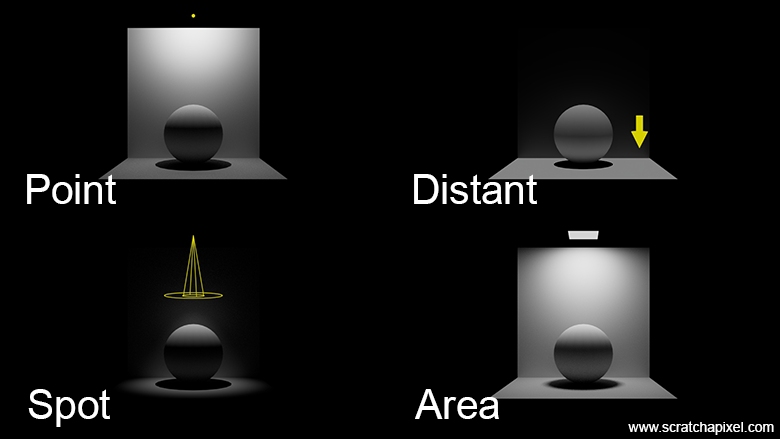
\includegraphics[width=\linewidth]{imagens/light_3.png}
			\end{center}
		\end{column}

		% --- RIGHT COLUMN ---
		\begin{column}{0.5\textwidth}
			\begin{center}
				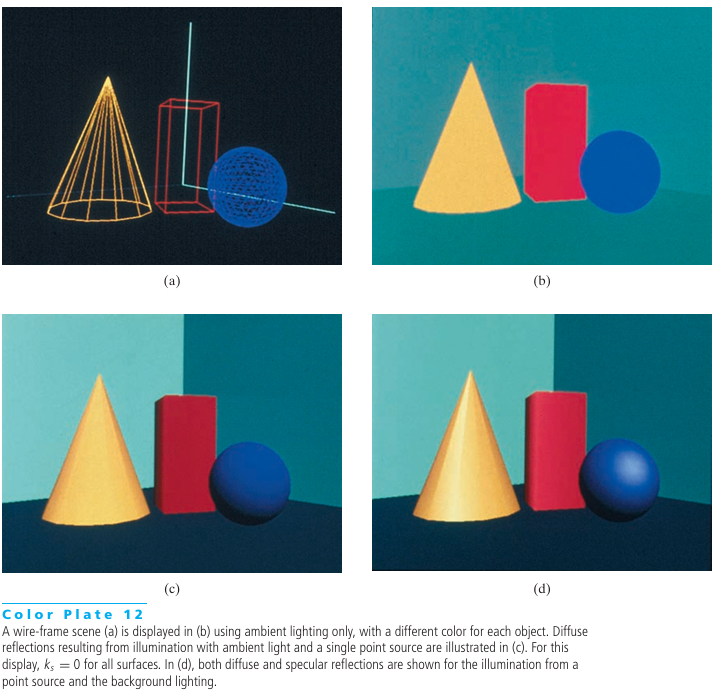
\includegraphics[width=\linewidth]{imagens/rendering_model_3.png}
			\end{center}
		\end{column}
	\end{columns}
\end{frame}

\begin{frame}{Bối cảnh}
	\begin{columns}[T]
		% --- LEFT COLUMN ---
		\begin{column}{0.5\textwidth}
			\begin{center}
				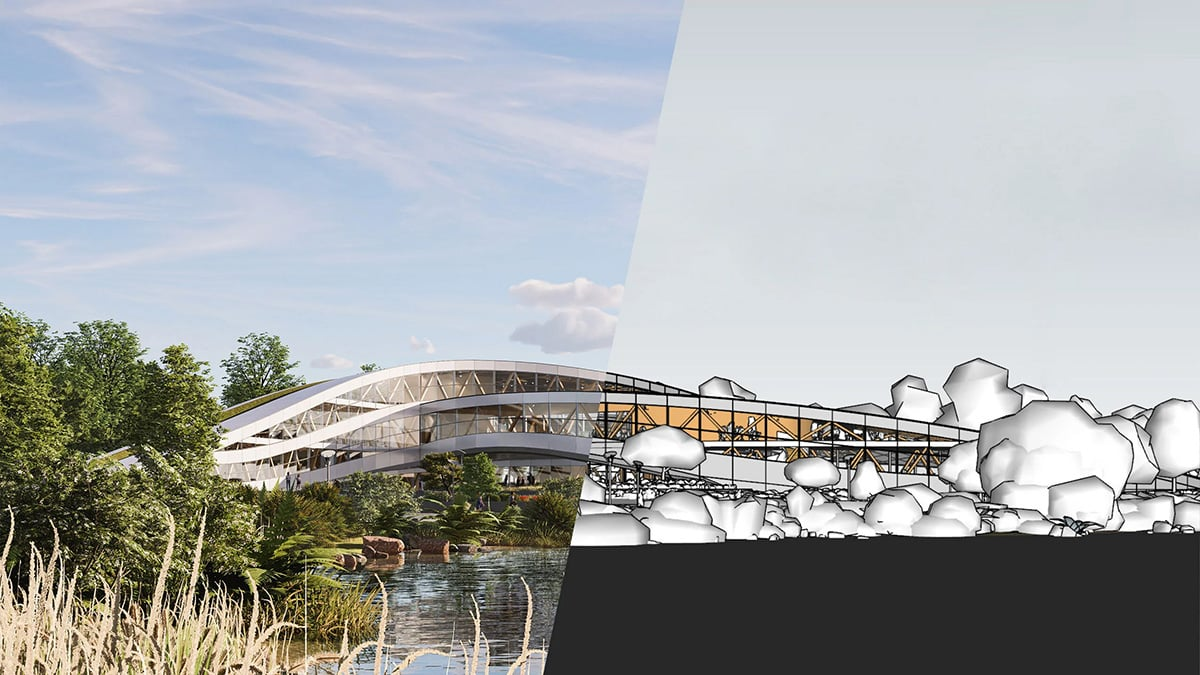
\includegraphics[width=\linewidth]{imagens/rendering_model_1.jpg}
				
			\end{center}
		\end{column}
		
		% --- RIGHT COLUMN ---
		\begin{column}{0.5\textwidth}
			\begin{center}
				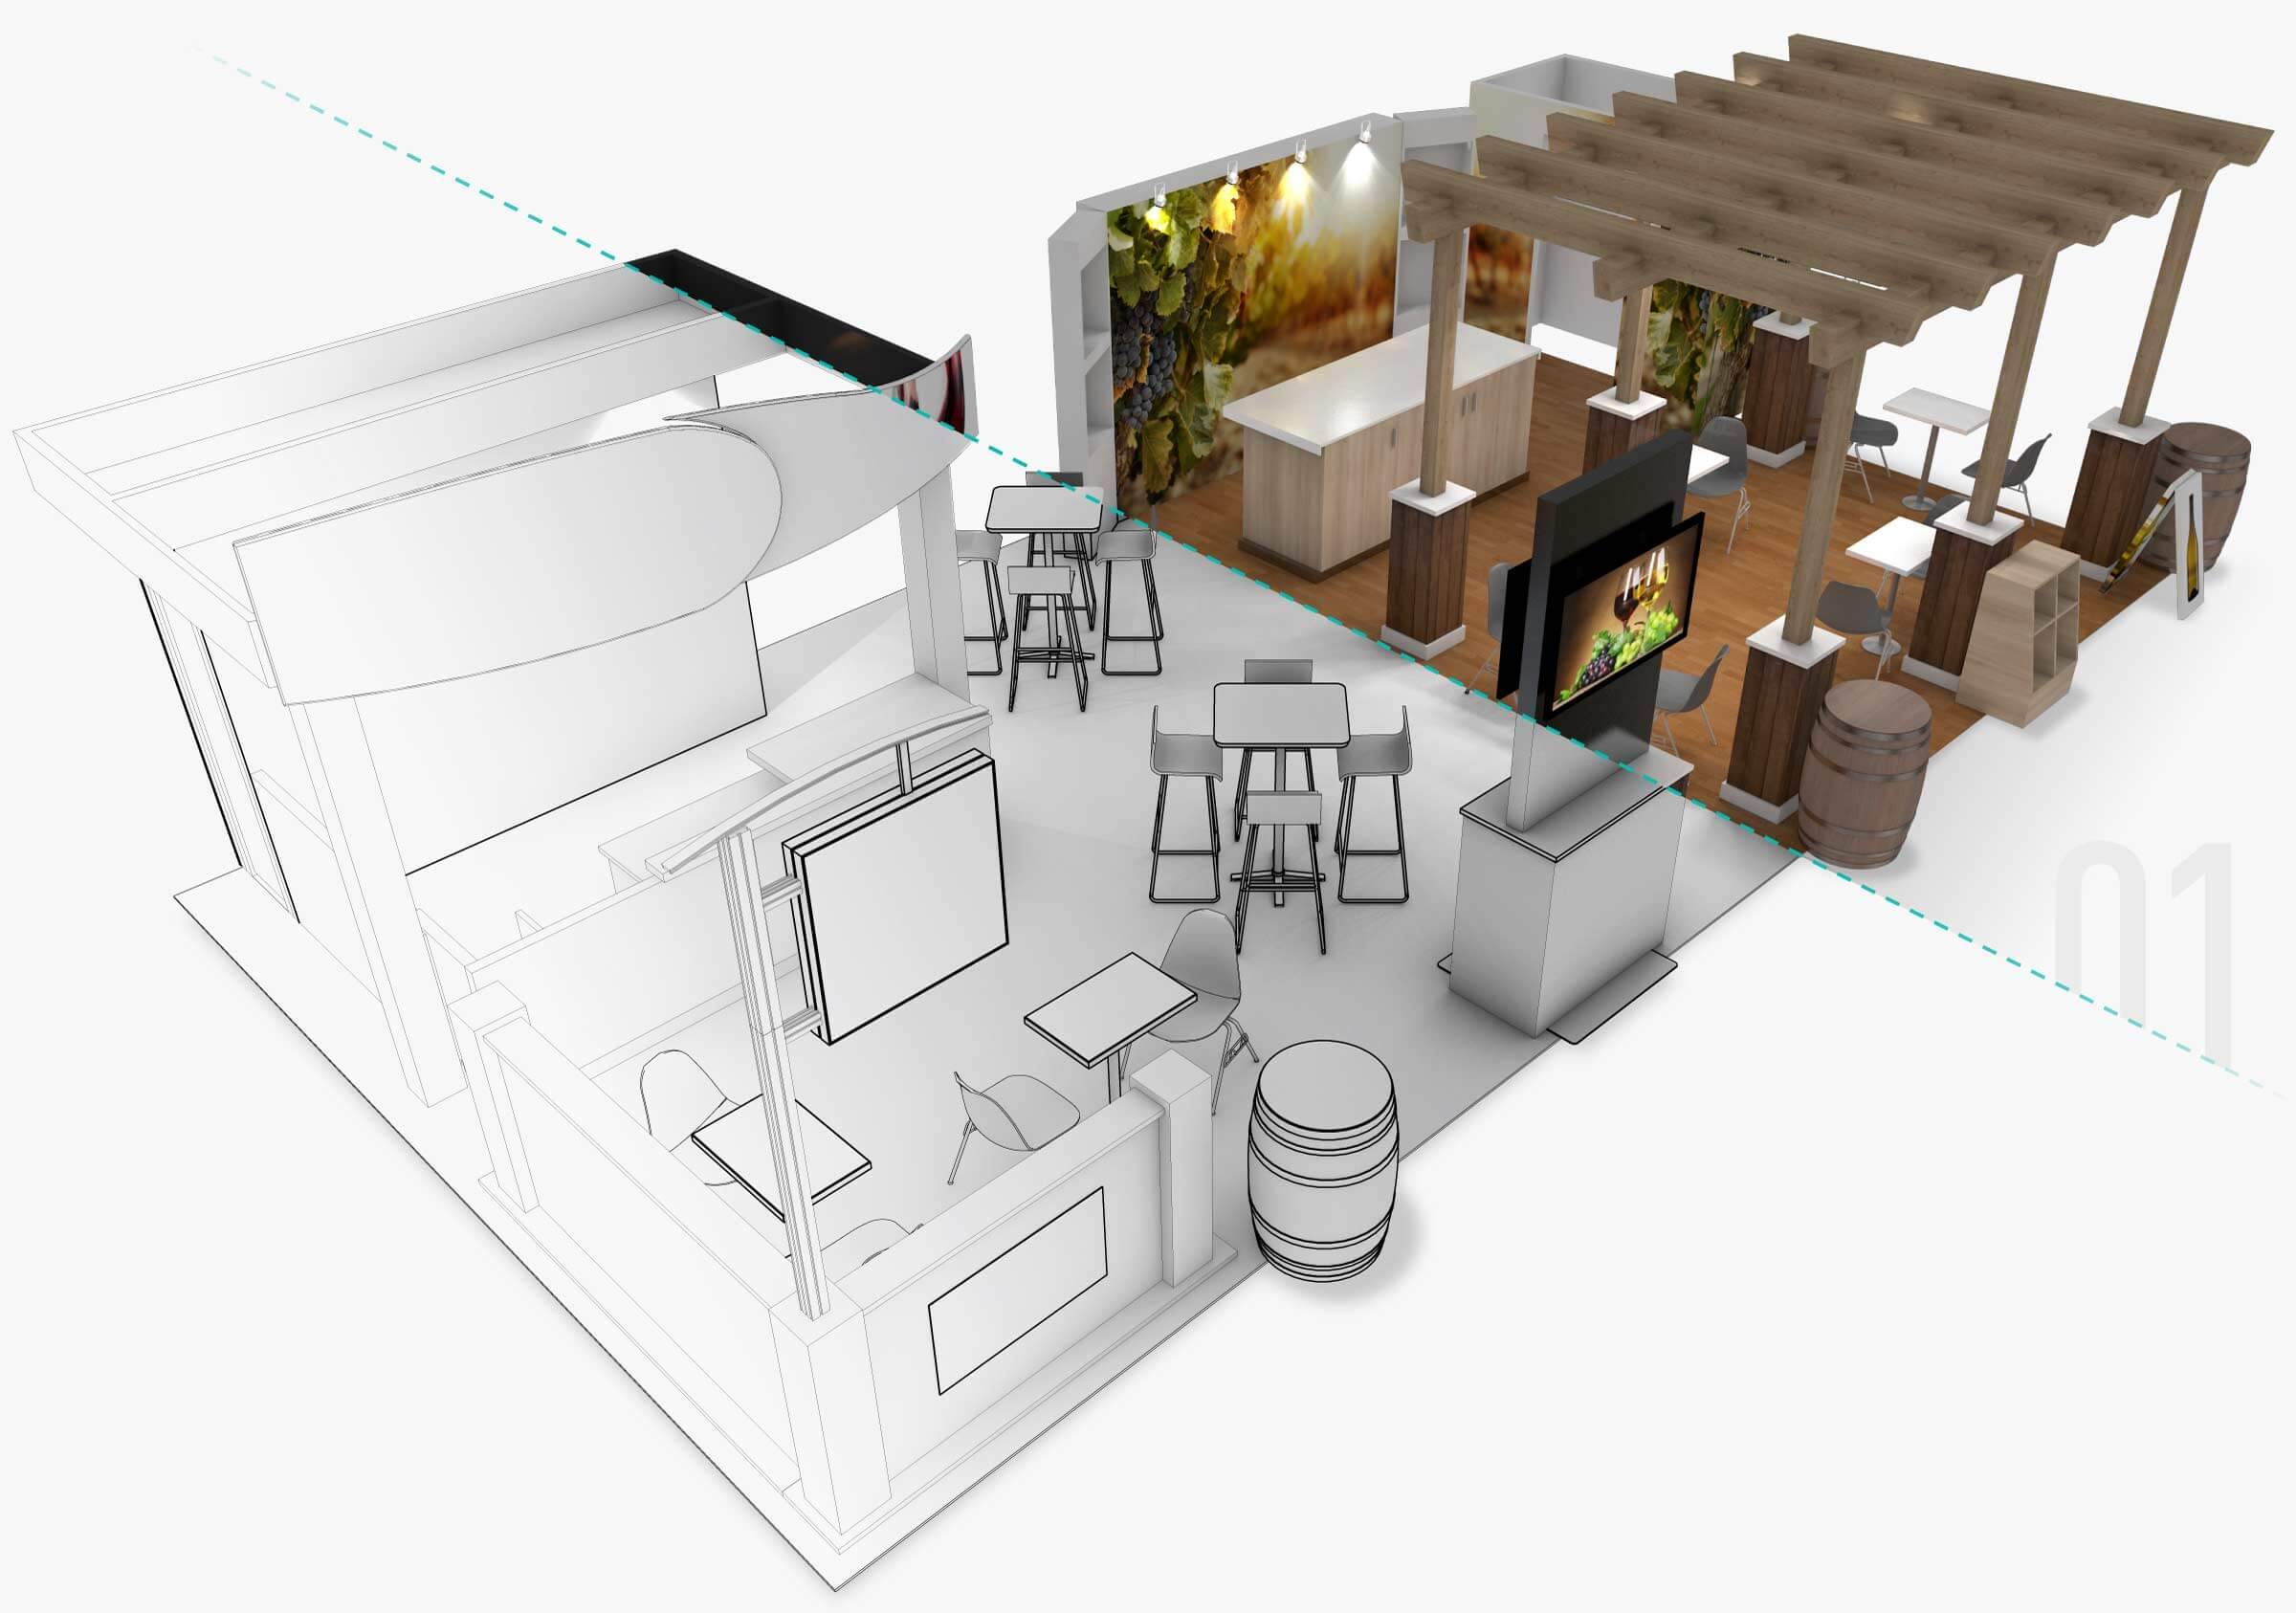
\includegraphics[width=\linewidth]{imagens/rendering_model_2.jpg}
			\end{center}
		\end{column}
	\end{columns}
\end{frame}

\begin{frame}{Bối cảnh}
	Sự phát triển của lĩnh vực này có thể được chia thành các giai đoạn sau:
	\begin{itemize}
		\item \textbf{Thập niên 1970 - Các mô hình thực nghiệm}
		\item \textbf{Thập niên 1980 - Cách mạng dựa trên vật lý}
		\item \textbf{Thập niên 2010 - Mô hình dựa trên học sâu}
	\end{itemize}
\end{frame}

\begin{frame}{Thập niên 1970 - Các mô hình thực nghiệm}
	Giai đoạn đầu của đồ họa máy tính hiện đại tập trung vào việc xây dựng các mô hình thực nghiệm nhằm tạo ra hình ảnh có tính thuyết phục thị giác với chi phí tính toán tối thiểu. \pause \\
	Các công trình tiêu biểu làm nền tảng:
	\begin{itemize}
		\item Gouraud Shading
		\item Phong Reflectance Model và Phong Shading
		\item Blinn-Phong Reflectance Model
	\end{itemize} \pause
	Mặc dù không mang tính chính xác vật lý, các mô hình này có ảnh hưởng sâu rộng và vẫn được sử dụng trong nhiều hệ thống kết xuất thời gian thực nhờ tính đơn giản và hiệu quả.
\end{frame}

\begin{frame}{Thập niên 1980 - Cách mạng dựa trên vật lý}
	Từ thập niên 1980, trọng tâm nghiên cứu dần chuyển sang việc mô phỏng sự tương tác ánh sáng toàn cục trong cảnh, hay còn gọi là chiếu sáng toàn cục (global illumination).
	
	Một cột mốc quan trọng là sự ra đời của \textit{Hàm phân phối phản xạ hai chiều} (Bidirectional Reflectance Distribution Function -- BRDF) vào năm 1982, cung cấp một khung toán học tổng quát để mô tả cách ánh sáng phản xạ trên bề mặt vật thể.
	
	Tiếp đó, \textit{Phương trình kết xuất} (The Rendering Equation) được giới thiệu năm 1986 đã thống nhất nhiều hiện tượng chiếu sáng trong một biểu thức toán học duy nhất, trở thành nền tảng lý thuyết cho hầu hết các thuật toán kết xuất quang thực hiện đại.
\end{frame}

\begin{frame}{Thập niên 2010 - Mô hình dựa trên học sâu}
	Trong thập niên gần đây, học sâu đã trở thành một hướng tiếp cận quan trọng, không chỉ nhằm tăng tốc các quy trình kết xuất truyền thống mà còn để tái định nghĩa bản chất của quá trình kết xuất.
\end{frame}

\begin{frame}{Thập niên 2010 - Mô hình dựa trên học sâu}
	Công trình đột phá nhất trong lĩnh vực này là \textit{Trường bức xạ thần kinh (Neural Radiance Fields - NeRF)} vào năm 2020. NeRF có khả năng tạo ra các góc nhìn mới với chất lượng quang thực ấn tượng từ một tập hợp hình ảnh đầu vào thưa thớt.
	\begin{columns}[T]
		% --- LEFT COLUMN ---
		\begin{column}{0.5\textwidth}
			\begin{center}
				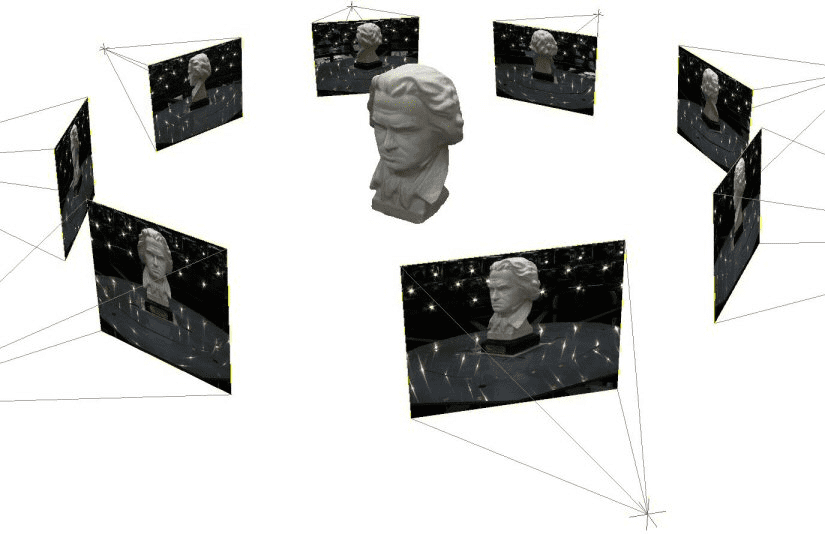
\includegraphics[width=\linewidth]{imagens/nerf_1.png}
				
			\end{center}
		\end{column}
		
		% --- RIGHT COLUMN ---
		\begin{column}{0.5\textwidth}
			\begin{center}
				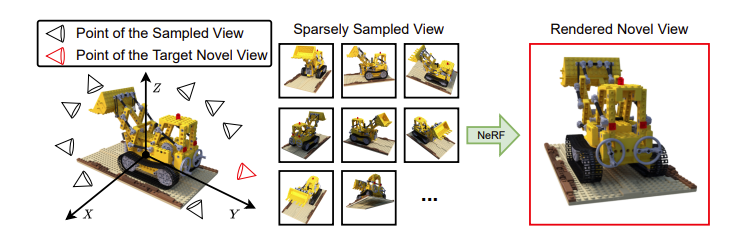
\includegraphics[width=\linewidth]{imagens/nerf_2.png}
			\end{center}
		\end{column}
	\end{columns}

\end{frame}

\subsection{Động lực nghiên cứu}
\begin{frame}{Động lực nghiên cứu}
	Mặc dù đồ họa máy tính hiện đại đã đạt đến mức độ quang thực rất cao, quá trình cải tiến công nghệ trong lĩnh vực này vẫn chưa dừng lại.
	
	Năng lực tính toán của các thiết bị phần cứng ngày càng tăng, trong khi chi phí sản xuất liên tục giảm, khiến đồ họa máy tính trở nên dễ tiếp cận hơn đối với cả nhà phát triển lẫn người dùng cuối. Song song với đó, kỳ vọng của người dùng về chất lượng hình ảnh, mức độ chân thực và khả năng tương tác cũng không ngừng gia tăng.
	
	Điều này tạo ra một động lực mạnh mẽ thúc đẩy nghiên cứu và phát triển các mô hình chiếu sáng và kỹ thuật kết xuất ngày càng chính xác và hiệu quả hơn.

\end{frame}

\begin{frame}{Động lực nghiên cứu}
	\textbf{Giải trí và truyền thông:} Trong ngành công nghiệp điện ảnh và trò chơi điện tử, tiêu chuẩn về chất lượng hình ảnh và mức độ đắm chìm của người dùng ngày càng cao. Việc nâng cao trải nghiệm nhập vai và cảm giác hiện diện trong không gian ảo trở thành mục tiêu then chốt để thu hút và giữ chân người dùng. Các kỹ thuật kết xuất tiên tiến, đặc biệt là dò tia thời gian thực, cho phép mô phỏng phản xạ, bóng đổ và chiếu sáng toàn cục phức tạp, góp phần nâng cao đáng kể tính chân thực và sức hấp dẫn của nội dung số.
\end{frame}

\begin{frame}{Động lực nghiên cứu}
	\begin{center}
		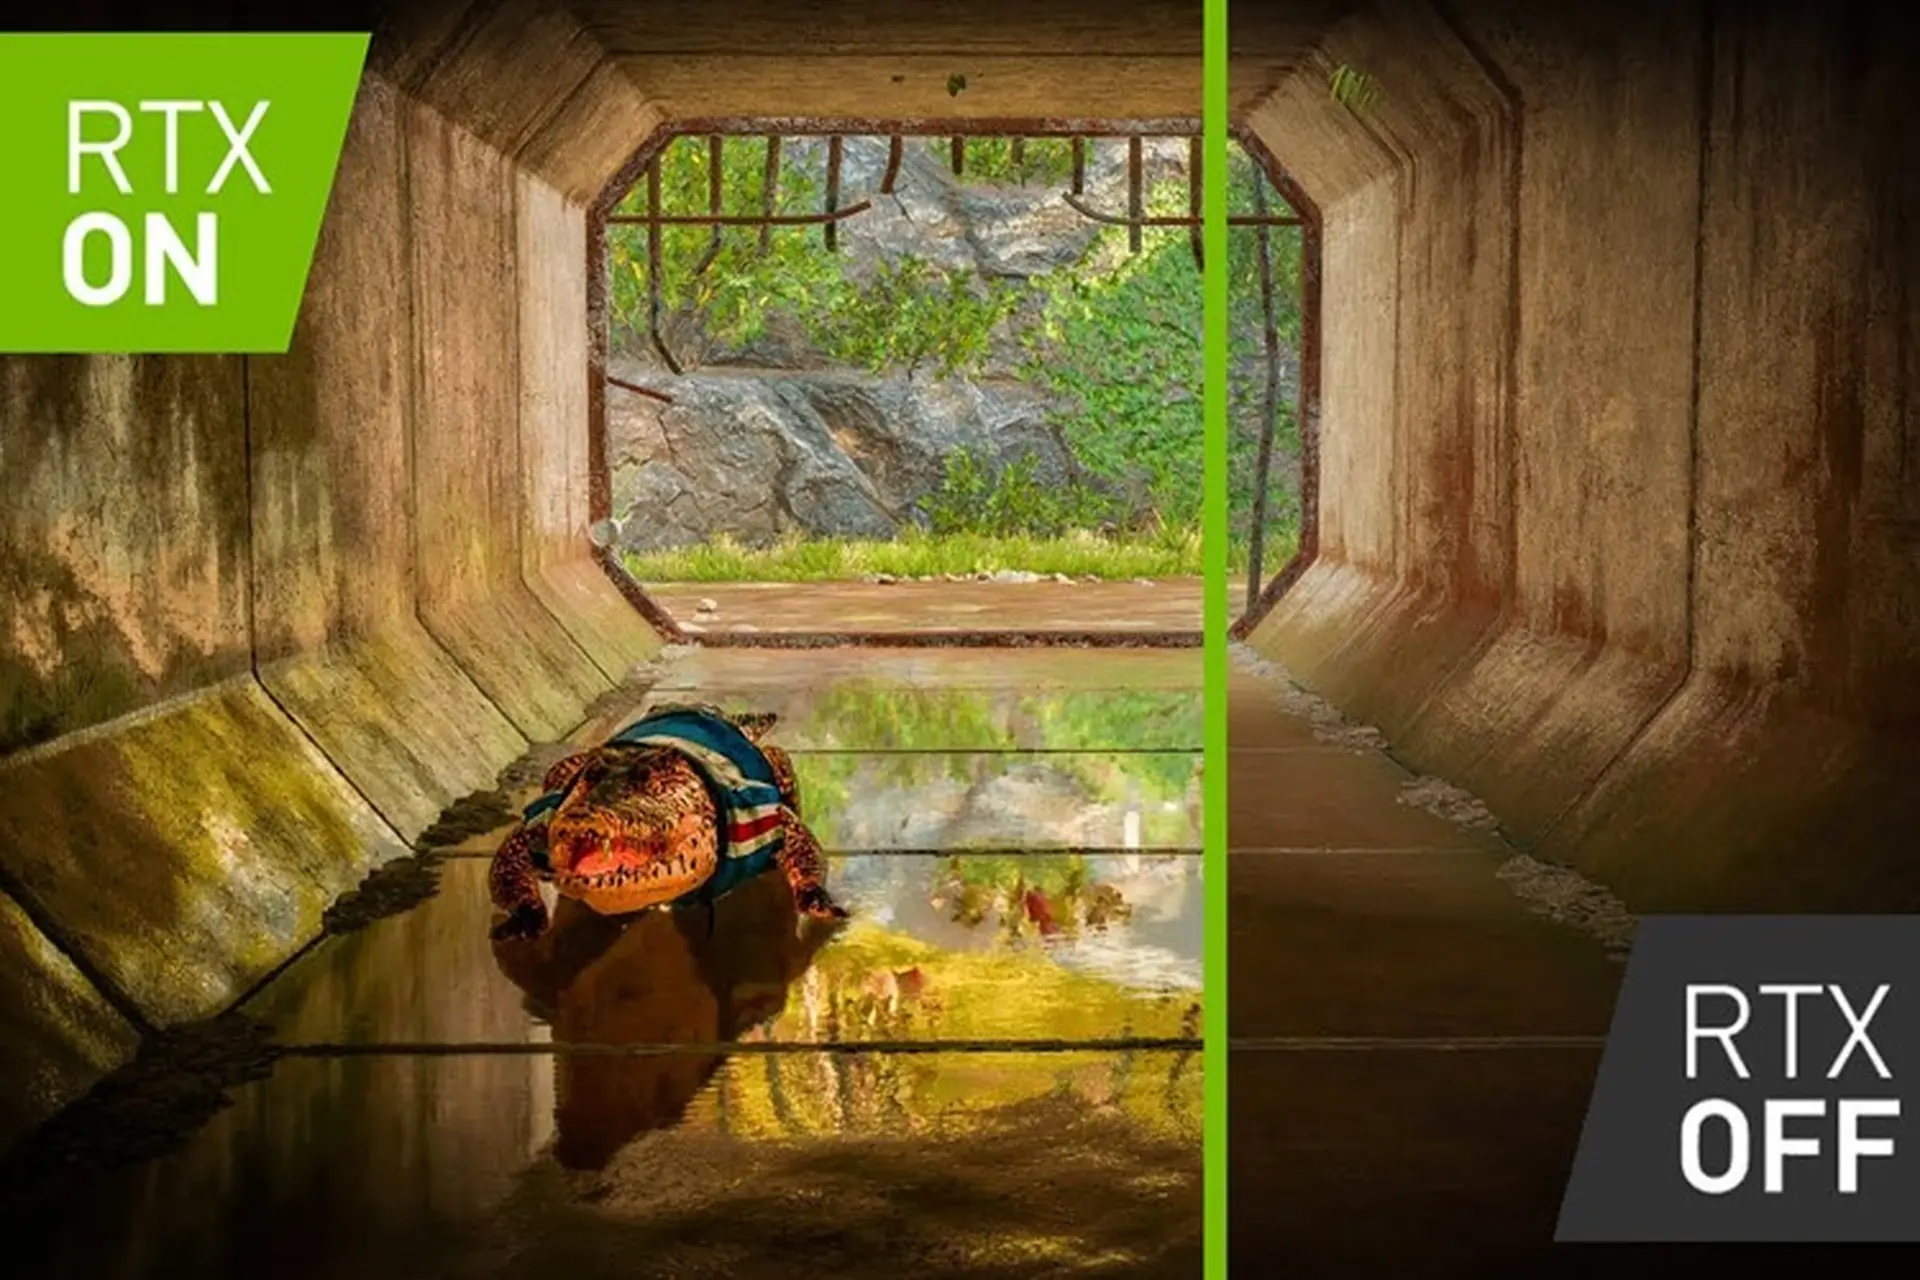
\includegraphics[height=0.23\linewidth]{imagens/rtx_3.png}
		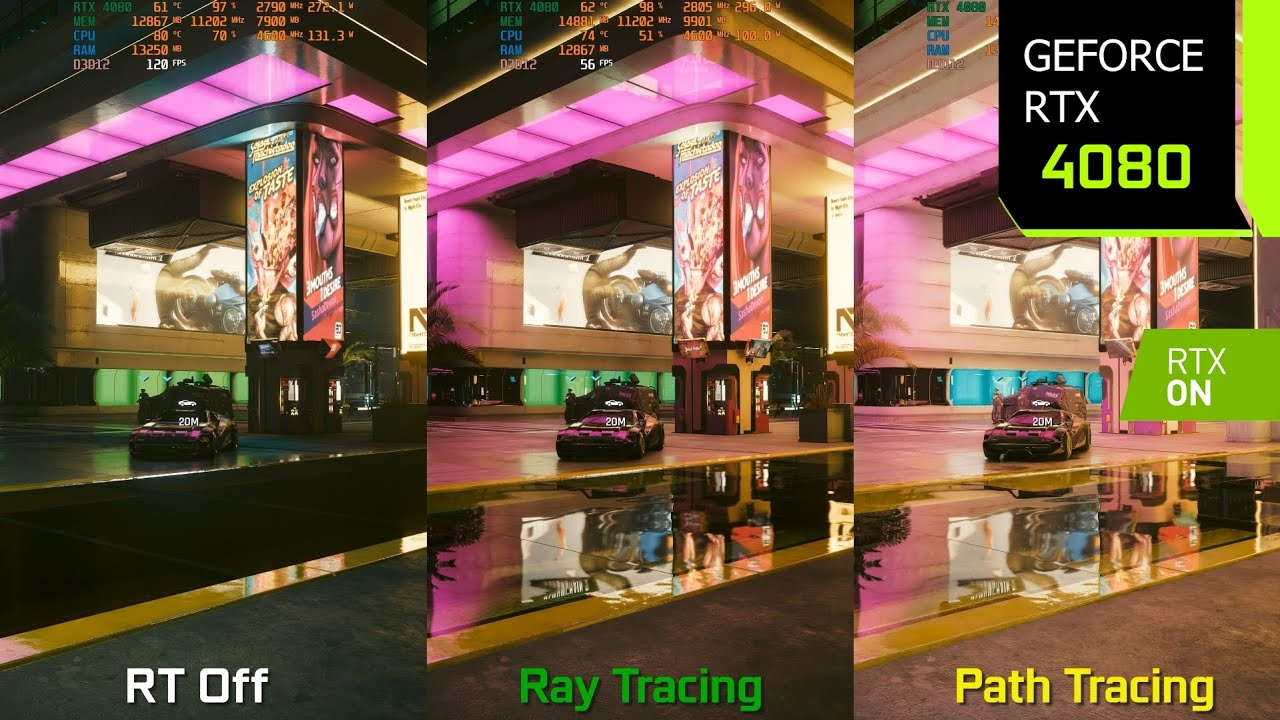
\includegraphics[height=0.23\linewidth]{imagens/rtx_4.jpg}\\
		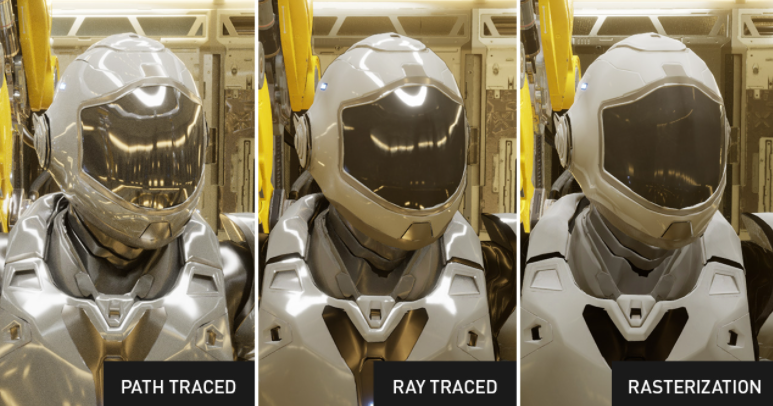
\includegraphics[height=0.23\linewidth]{imagens/rtx_5.png}
	\end{center}
\end{frame}

\begin{frame}{Động lực nghiên cứu}
	\textbf{Kỹ thuật, kiến trúc và thiết kế:} Các mô hình chiếu sáng có độ chính xác vật lý cao cho phép kiến trúc sư và kỹ sư đánh giá tác động của ánh sáng tự nhiên và nhân tạo trong các công trình ở những điều kiện khác nhau. Nhờ đó, các quyết định thiết kế có thể được đưa ra dựa trên mô phỏng đáng tin cậy thay vì chỉ dựa vào kinh nghiệm. Trong thiết kế công nghiệp, việc kết xuất đối tượng với vật liệu và ánh sáng chân thực giúp mô phỏng sản phẩm trước khi chế tạo, góp phần giảm chi phí và thời gian cho các giai đoạn thử nghiệm.
\end{frame}

\begin{frame}{Động lực nghiên cứu}
	\begin{columns}[T]
		% --- LEFT COLUMN ---
		\begin{column}{0.5\textwidth}
			\begin{center}
				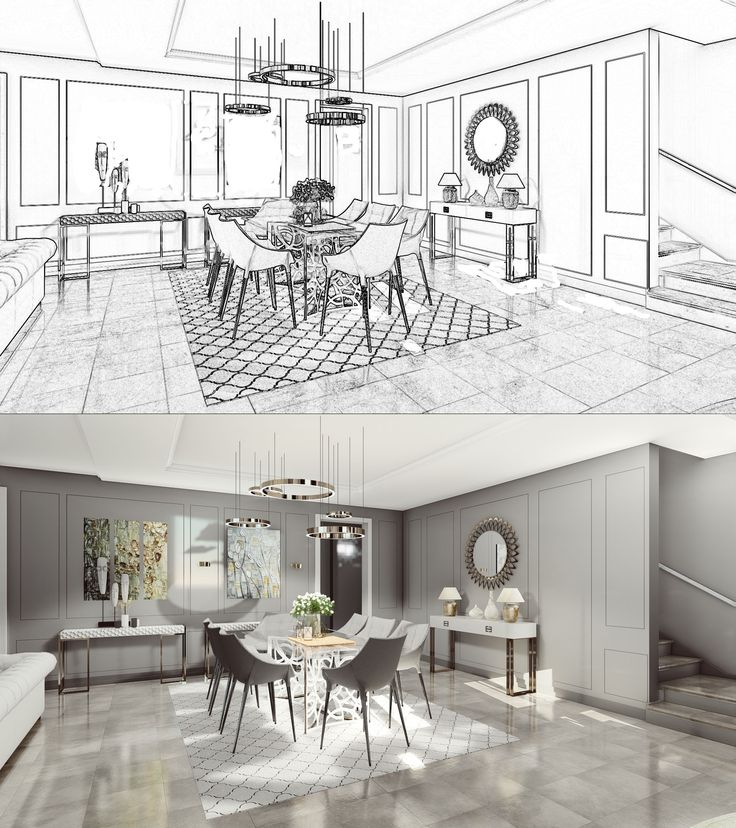
\includegraphics[height=0.8\linewidth]{imagens/architecture_2.jpg}
				
			\end{center}
		\end{column}
		
		% --- RIGHT COLUMN ---
		\begin{column}{0.5\textwidth}
			\begin{center}
				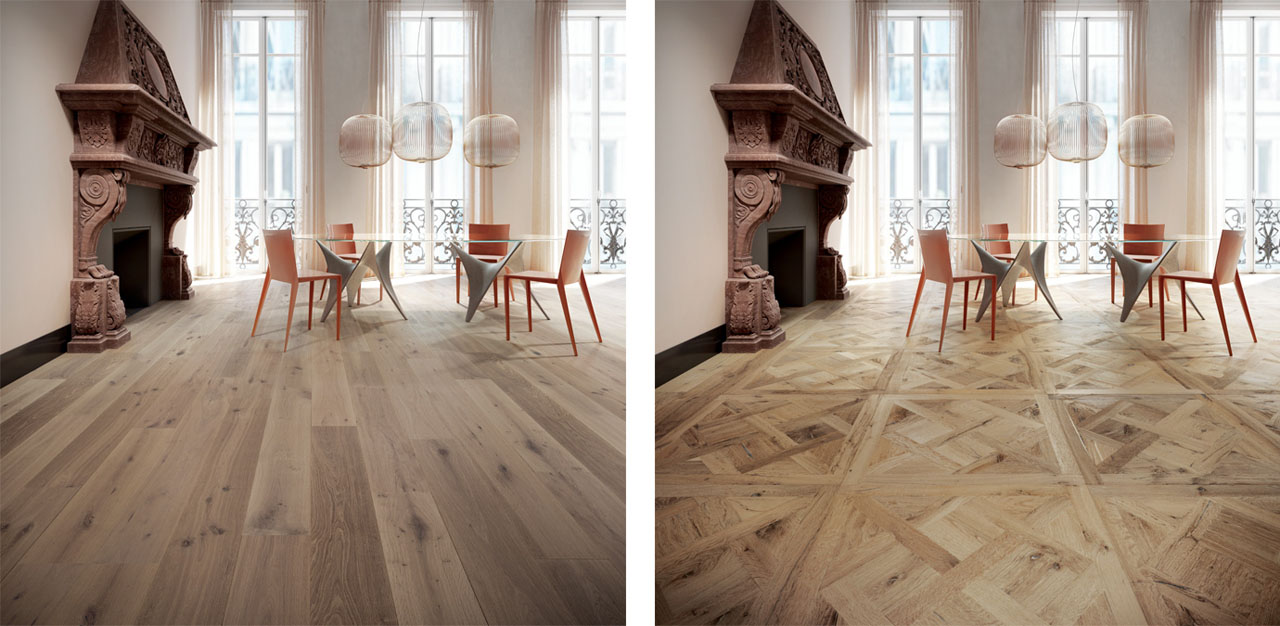
\includegraphics[width=\linewidth]{imagens/architecture_5.jpg}
			\end{center}
		\end{column}
	\end{columns}
\end{frame}

\begin{frame}{Động lực nghiên cứu}
	\begin{columns}[T]
		% --- LEFT COLUMN ---
		\begin{column}{0.5\textwidth}
			\begin{center}
				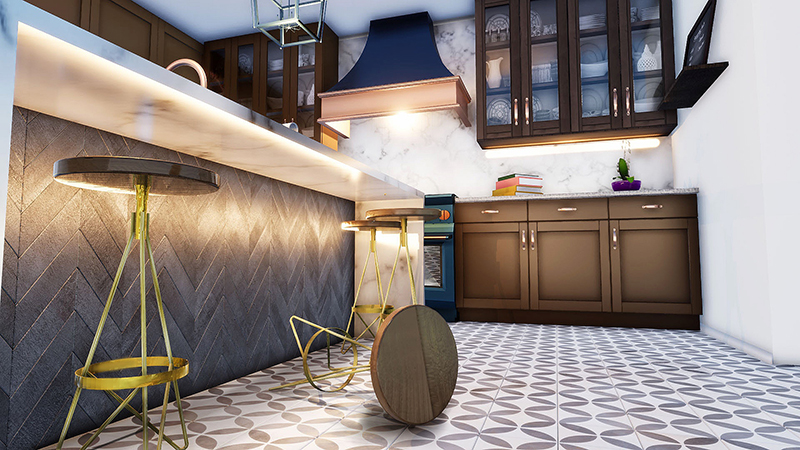
\includegraphics[width=\linewidth]{imagens/architecture_3.jpg}
				
			\end{center}
		\end{column}
		
		% --- RIGHT COLUMN ---
		\begin{column}{0.5\textwidth}
			\begin{center}
				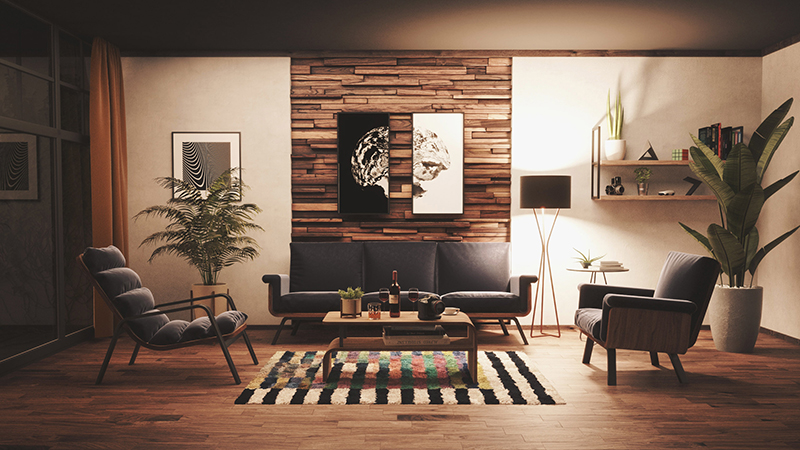
\includegraphics[width=\linewidth]{imagens/architecture_4.jpg}
			\end{center}
		\end{column}
	\end{columns}
\end{frame}

\begin{frame}{Động lực nghiên cứu}
	\begin{center}
		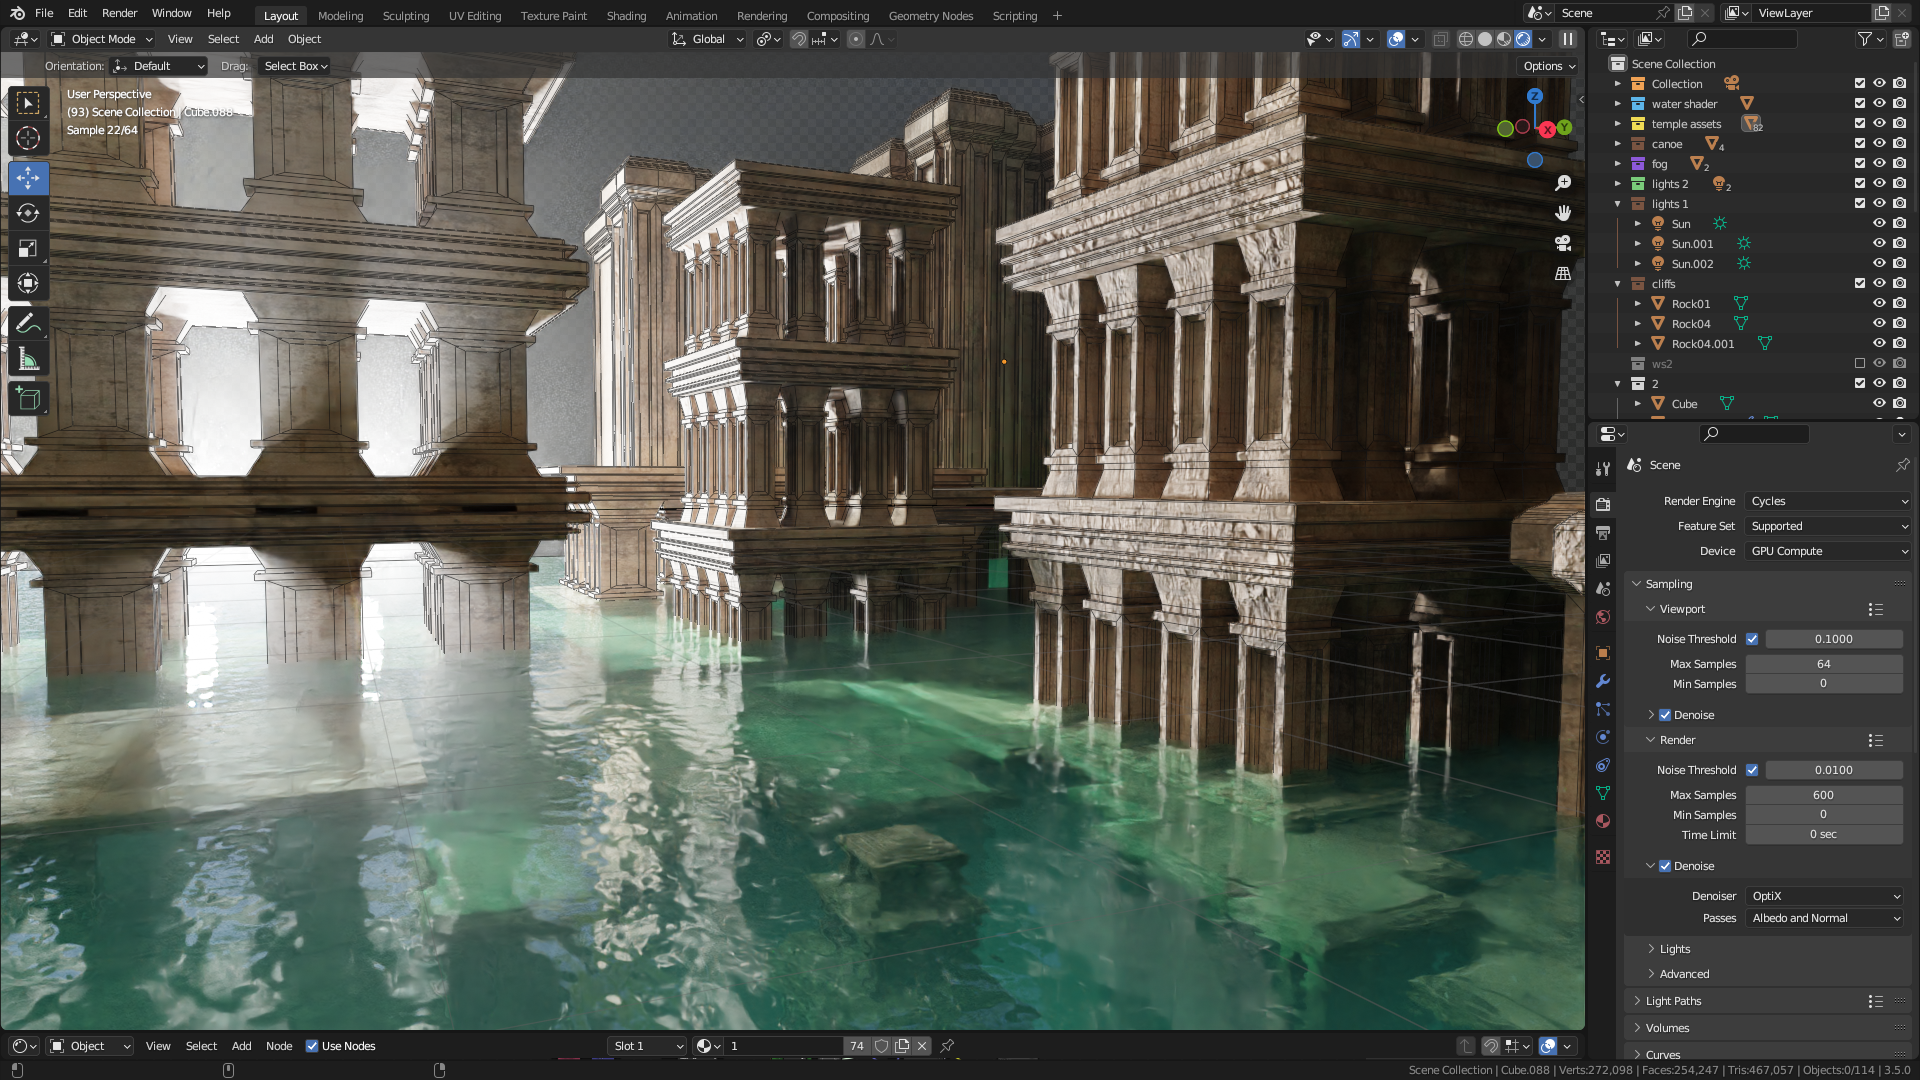
\includegraphics[width=0.8\linewidth]{imagens/rtx_6.png}
	\end{center}
\end{frame}

\begin{frame}{Động lực nghiên cứu}
	\textbf{Khoa học:} Trong lĩnh vực y học, các kỹ thuật như kết xuất thể tích cho phép tái tạo và quan sát các cấu trúc bên trong cơ thể từ dữ liệu hai chiều như CT hoặc MRI, hỗ trợ chẩn đoán và lập kế hoạch điều trị. Trong các ngành khoa học khác, việc trực quan hóa các tập dữ liệu phức tạp đòi hỏi các mô hình chiếu sáng có khả năng làm nổi bật những chi tiết hình học nhỏ hoặc các cấu trúc khó quan sát, từ đó giúp nhà nghiên cứu hiểu rõ hơn bản chất của hiện tượng được mô phỏng.
\end{frame}

\subsection{Ý nghĩa khoa học}
\begin{frame}{Ý nghĩa khoa học}
	Phương trình kết xuất do Kajiya đề xuất là nền tảng lý thuyết cho hầu hết các trình kết xuất hiện đại, tuy nhiên phương trình này không có lời giải giải tích trong hầu hết các trường hợp thực tế phức tạp. Do đó, việc phát triển các thuật toán số hiệu quả nhằm xấp xỉ lời giải của phương trình kết xuất, chẳng hạn như \textit{Vận chuyển ánh sáng Metropolis} (Metropolis Light Transport) hay \textit{Ước tính mật độ photon tiến bộ} (Progressive Photon Mapping), vẫn là một hướng nghiên cứu tích cực và có ý nghĩa lâu dài.
\end{frame}

\begin{frame}{Ý nghĩa khoa học}
	Sự phát triển của các kỹ thuật như NeRF mở ra một hướng đi hoàn toàn mới. Thay vì mô phỏng vật lý một cách tường minh, các mô hình này học một biểu diễn ngầm của cảnh từ dữ liệu. 
	
	Với xu hướng phát triển trí tuệ nhân tạo khả diễn giải (xAI), đã thúc đẩy việc tìm hiểu các giới hạn và khả năng của những biểu diễn ngầm này. Các câu hỏi đặt ra bao gồm việc làm thế nào để đảm bảo các mô hình học máy tuân thủ các định luật vật lý, cũng như khả năng sử dụng mạng nơ-ron để đề xuất các phương pháp mới nhằm cải thiện việc mô phỏng ánh sáng trong không gian ba chiều.
\end{frame}

\subsection{Ý nghĩa thực tiễn}
\begin{frame}{Ý nghĩa thực tiễn}
	Rào cản lớn nhất đối với việc áp dụng rộng rãi các kỹ thuật quang thực là chi phí tính toán. Mục tiêu nghiên cứu nhằm tập trung vào việc phát triển các thuật toán xấp xỉ thông minh, các cấu trúc dữ liệu hiệu quả, và tận dụng khả năng xử lý song song của phần cứng hiện đại (GPU) để đưa chất lượng hình ảnh ngoại tuyến (offline) vào các ứng dụng tương tác thời gian thực.
\end{frame}

\begin{frame}{Ý nghĩa thực tiễn}
	Sự phát triển của thực tế tăng cường (AR), thực tế ảo (VR), thực tế hỗn hợp (MR) và vũ trụ ảo (Metaverse) đòi hỏi khả năng kết xuất các thế giới số phức tạp, liên tục và hiệu quả trên các thiết bị có tài nguyên hạn chế. Điều này tạo ra một nhu cầu cho các mô hình chiếu sáng và thuật toán kết xuất vừa nhẹ, vừa có độ thực tế cao.
\end{frame}

\subsection{Phát biểu bài toán}
\begin{frame}{Phát biểu bài toán}
	Bài toán tổng hợp hình ảnh trong đồ họa máy tính có thể được mô tả như quá trình ánh xạ một mô tả toán học trừu tượng của một cảnh ba chiều sang một biểu diễn hai chiều dưới dạng hình ảnh số. Mục tiêu của quá trình này là tạo ra một hình ảnh đầu ra có mức độ chân thực cao, sao cho trong giới hạn nhận thức thị giác của con người, hình ảnh đó không thể hoặc khó phân biệt với một bức ảnh chụp của một cảnh tương tự trong thế giới thực.
\end{frame}

\begin{frame}{Phát biểu bài toán}
	Mô hình chiếu sáng là một mô hình toán học, ký hiệu là $\textbf{f}$, mô tả cách ánh sáng tương tác với vật chất tại một điểm trên bề mặt vật thể. Cụ thể, với một điểm bề mặt $p$, hàm $\textbf{f}$ nhận vào thông tin hình học, vật liệu, chiếu sáng và hướng quan sát, và trả về lượng bức xạ hoặc giá trị màu được phản xạ từ điểm $p$ theo hướng quan sát đó. Do đó, $\textbf{f}$ quyết định màu sắc cục bộ tại từng điểm nhìn thấy trong cảnh.
\end{frame}

\begin{frame}{Phát biểu bài toán}
	Quá trình kết xuất đối tượng là một thuật toán hoặc một hệ thống, ký hiệu là $\textbf{R}$, có nhiệm vụ tổng hợp hình ảnh hai chiều cuối cùng từ một mô tả cảnh hoàn chỉnh. Hàm kết xuất $\textbf{R}$ đóng vai trò là cơ chế toàn cục, chịu trách nhiệm tổ chức và thực thi việc đánh giá hàm $\textbf{f}$ trên toàn bộ cảnh. Hàm $\textbf{R}$ xác định, đối với mỗi điểm ảnh trên mặt phẳng ảnh, điểm tương ứng trên bề mặt các đối tượng trong cảnh, cũng như các điều kiện quan sát và chiếu sáng cần thiết. Trên cơ sở đó, $\textbf{R}$ gọi và tổng hợp kết quả của hàm $\textbf{f}$ để tính toán giá trị màu cuối cùng cho từng điểm ảnh.
\end{frame}


\begin{frame}{Phát biểu bài toán}
	\textbf{Input:} Một mô tả cảnh ba chiều (3D Scene Description) hoàn chỉnh dưới dạng dữ liệu số. Dữ liệu này bao gồm:
	\begin{enumerate}
		\item \textbf{Hình học (Geometry -- $G$):} Mô tả hình dạng, vị trí và cấu trúc không gian của các đối tượng trong cảnh.
		\item \textbf{Vật liệu (Materials -- $M$):} Các tham số bề mặt xác định đặc tính phản xạ và tán xạ ánh sáng của mỗi đối tượng.
		\item \textbf{Chiếu sáng (Lighting -- $L$):} Mô tả các nguồn sáng trong cảnh, bao gồm vị trí, phổ năng lượng và cường độ.
		\item \textbf{Camera (Camera -- $C$):} Vị trí, hướng và các tham số quang học của camera ảo, xác định góc nhìn và miền quan sát của cảnh.
	\end{enumerate}
\end{frame}

\begin{frame}{Phát biểu bài toán}
	\textbf{Output:} Một hình ảnh hai chiều. Mỗi điểm ảnh (pixel) trên hình ảnh 2 chiều này chứa một giá trị màu, là kết quả của việc mô phỏng cách ánh sáng từ các nguồn sáng trong cảnh tương tác với các vật thể và cuối cùng đi đến "cảm biến" của camera ảo.\\
	\begin{gather*}
		x_{ij} = \textbf{f}(p_{ij}, G, M, L, C), \\
		Output = \textbf{R}(X), \quad X = \{ x_{ij} \mid i, j \in \Omega \},
	\end{gather*}
\end{frame}

\begin{frame}{Framework bài toán}
	\begin{enumerate}
		\item \textbf{Thiết lập không gian và hệ quy chiếu:} Xây dựng mô tả cảnh ba chiều và thiết lập các hệ tọa độ cần thiết, bao gồm không gian mô hình, không gian thế giới và không gian camera.
		
		\item \textbf{Xác định miền quan sát:} Thiết lập vị trí và hướng của camera, đồng thời xác định những phần của cảnh có khả năng đóng góp vào hình ảnh cuối cùng.
		
		\item \textbf{Ánh xạ hình học và phép chiếu:} Thực hiện các phép biến đổi hình học và phép chiếu nhằm ánh xạ các đối tượng từ không gian ba chiều sang miền hình ảnh hai chiều.
	\end{enumerate}
\end{frame}

\begin{frame}{Framework bài toán}
	\begin{enumerate}
		\item \textbf{Tính toán chiếu sáng và tô bóng:} Áp dụng mô hình chiếu sáng để tính toán lượng bức xạ đóng góp vào mỗi điểm ảnh, có thể bao gồm các hiệu ứng như bóng đổ, phản xạ, khúc xạ và chiếu sáng toàn cục.
		
		\item \textbf{Tổng hợp và hậu xử lý hình ảnh:} Thu thập các giá trị màu đã tính toán để tạo thành hình ảnh hai chiều hoàn chỉnh, đồng thời thực hiện các bước hiệu chỉnh cần thiết cho thiết bị hiển thị.
	\end{enumerate}
\end{frame}

\section{Các công trình nghiên cứu liên quan}
\subsection{Mô hình chiếu sáng}
\begin{frame}{Mô hình chiếu sáng}
	Trong thế giới vật lý, ánh sáng có thể được xem như dòng năng lượng điện từ lan truyền trong không gian và tương tác với vật chất thông qua các quá trình hấp thụ, phản xạ và tán xạ. Con người quan sát được các vật thể là nhờ ánh sáng từ các nguồn phát xạ tự nhiên hoặc nhân tạo chiếu tới bề mặt vật thể, sau đó một phần năng lượng được phản xạ về phía mắt, thông qua các tế bào thụ cảm ánh sáng (photoreceptor) chuyển đổi ánh sáng thành tín hiệu điện hoá, gửi đến não để tạo ra hình ảnh thị giác.
\end{frame}

\begin{frame}{Mô hình chiếu sáng}
	\begin{center}
		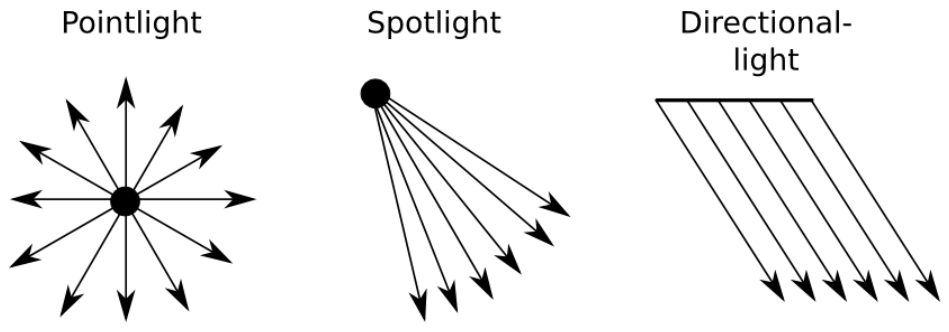
\includegraphics[height=0.3\linewidth]{imagens/light_1.png}
	\end{center}
\end{frame}

\begin{frame}{Mô hình chiếu sáng}
	\textbf{Nguồn sáng hình học - Geometric Light}\\
	Nguồn sáng hình học là các nguồn sáng được gán một vị trí cụ thể trong cảnh ba chiều. Cường độ ánh sáng phát ra từ các nguồn này suy giảm theo khoảng cách tới bề mặt được chiếu sáng, phản ánh quy luật lan truyền năng lượng trong không gian.
	
	Về mặt toán học, các nguồn sáng hình học thường được đặc trưng bởi:
	\begin{itemize}
		\item Vị trí không gian $p_i$.
		\item Cường độ phát xạ $I_i$.
		\item Hàm suy giảm theo khoảng cách \textit{attenuation} $f_{att}(r)$.
	\end{itemize}
\end{frame}


\begin{frame}{Nguồn sáng hình học}
	\textbf{Nguồn sáng điểm - Point Light}\\
	Nguồn sáng điểm là mô hình đơn giản nhất của nguồn sáng hình học, trong đó ánh sáng được phát ra đồng đều theo mọi hướng từ một điểm trong không gian. Mô hình này thường được sử dụng để xấp xỉ các nguồn sáng nhỏ như bóng đèn.
	
	Đóng góp ánh sáng tại một điểm bề mặt $x$ được tính như sau:
	\begin{gather*}
		I_o(x) = I_i * f_{att}(r) * max(0, n \cdot l)
	\end{gather*}
	trong đó:
	\begin{gather*}
		f_{att}(r) = \frac{1}{k_c + k_l * r + k_q * r^2}, \quad
		l = \frac{(p_i - x)}{||p_i - x||}
	\end{gather*}
	với $r = ||p_i - x||, n$ là vector pháp tuyến bề mặt tại $x$, và các hệ số $k_c, k_l, k_q$ điều chỉnh mức suy giảm cường độ theo khoảng cách.
\end{frame}

\begin{frame}{Nguồn sáng hình học}
	\begin{center}
		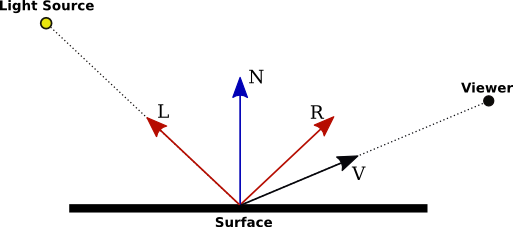
\includegraphics[height=0.45\textheight]{imagens/light-equation.png}
	\end{center}
\end{frame}

\begin{frame}{Nguồn sáng hình học}
	\begin{center}
		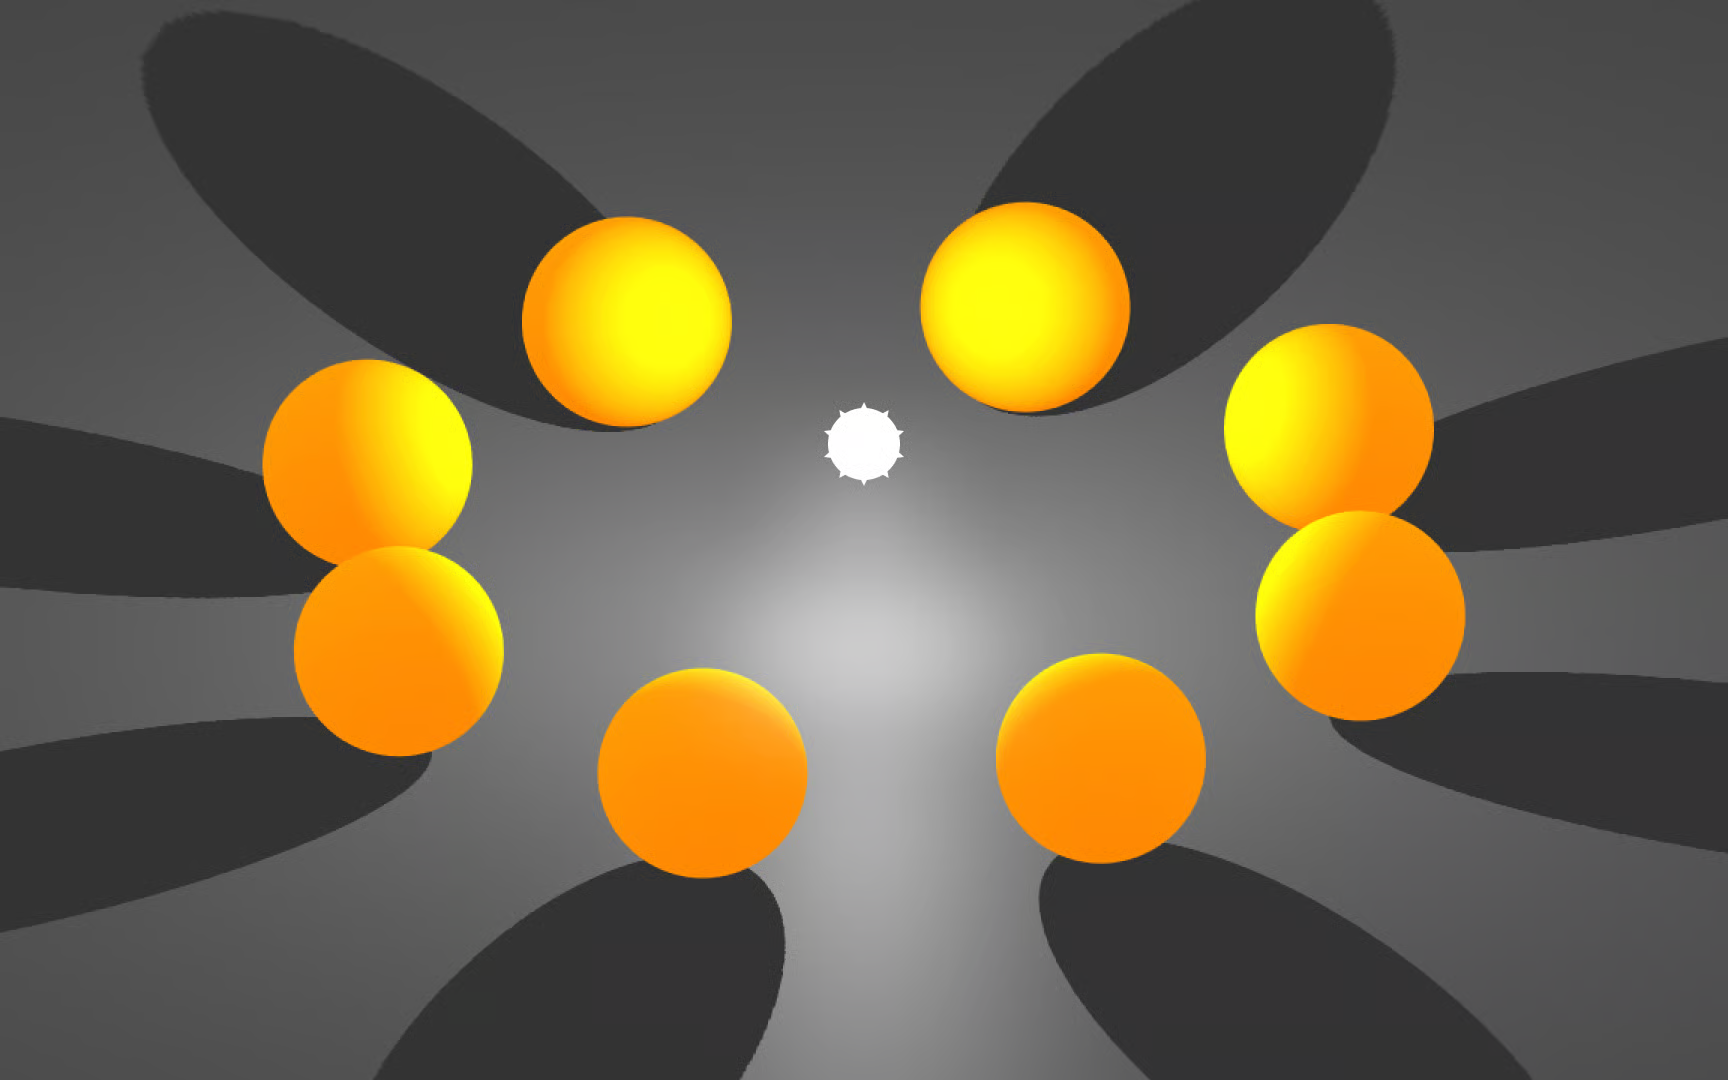
\includegraphics[height=0.45\textheight]{imagens/pointlight_1.png}
		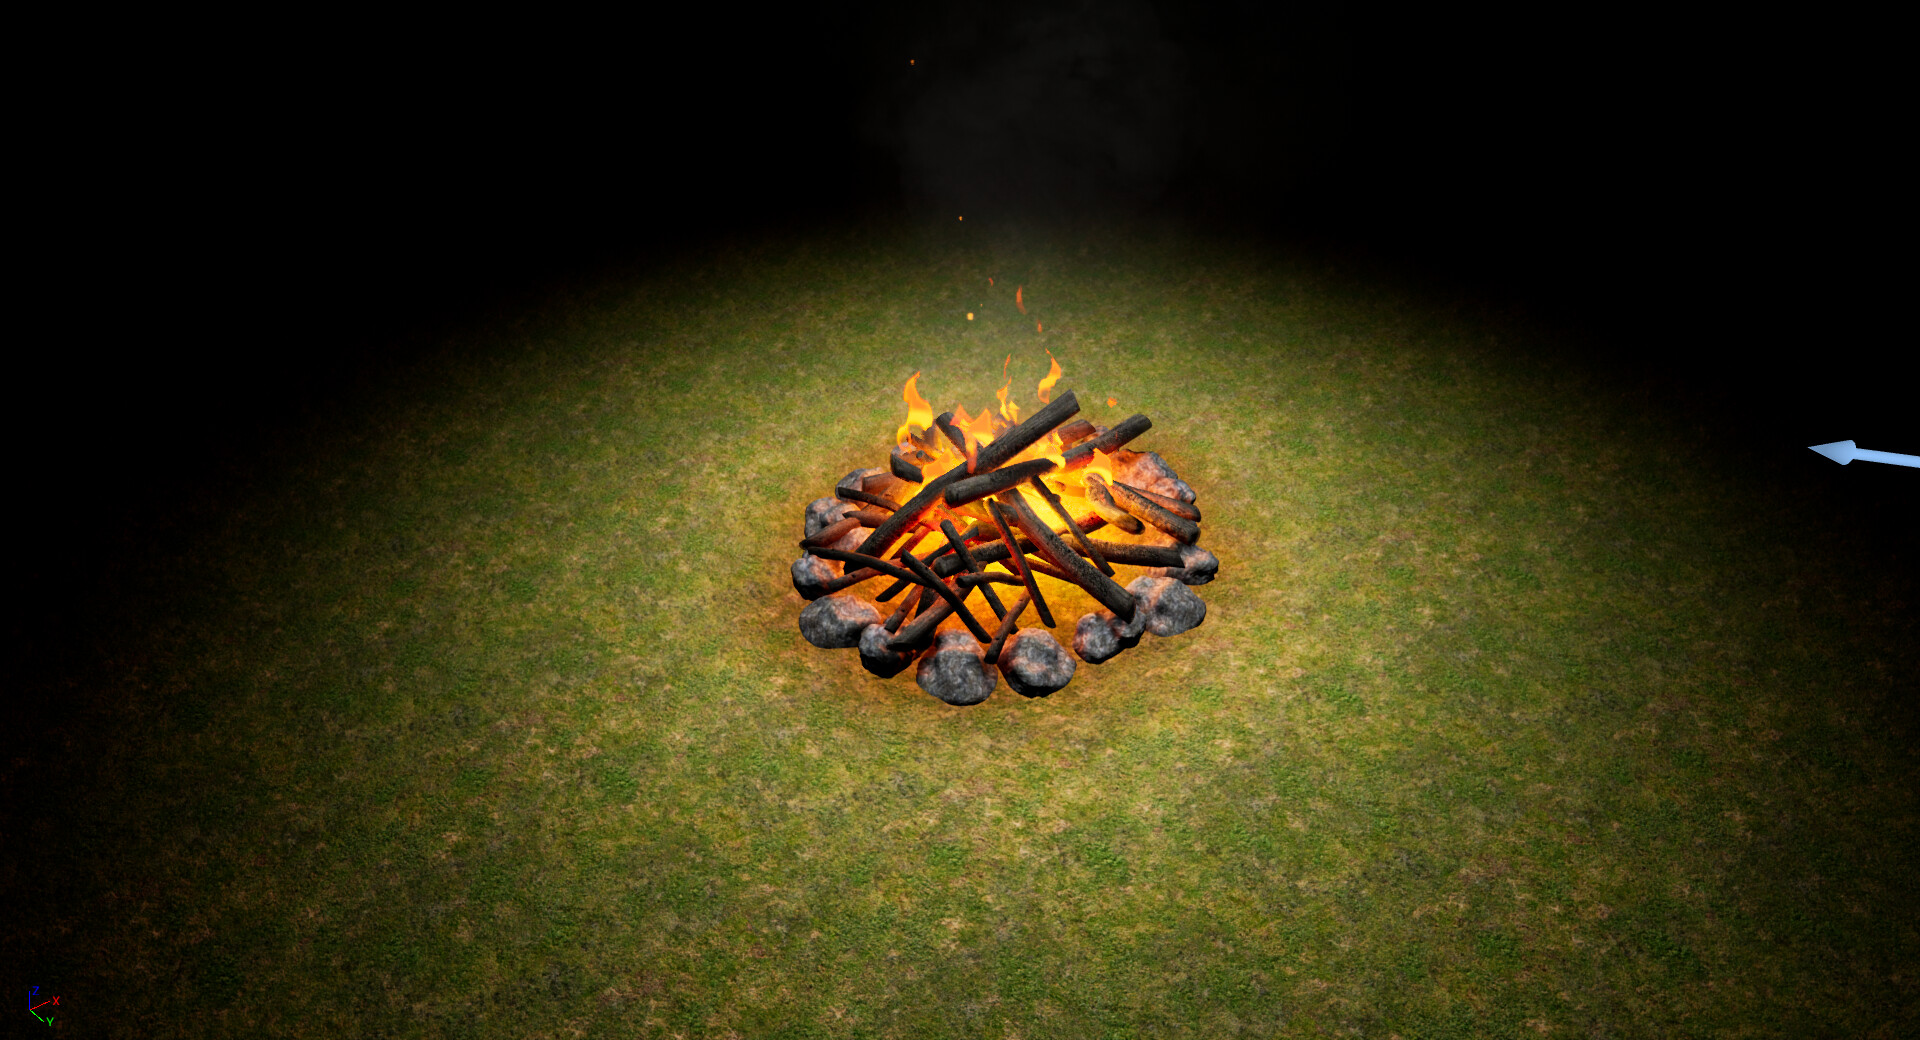
\includegraphics[height=0.45\textheight]{imagens/pointlight_2.jpg}
	\end{center}
\end{frame}

\begin{frame}{Nguồn sáng hình học}
	\textbf{Nguồn sáng chiếu điểm - Spot Light}\\
	Nguồn sáng chiếu điểm mở rộng mô hình nguồn sáng điểm bằng cách giới hạn vùng chiếu sáng trong một hình nón, mô phỏng các nguồn sáng có hướng rõ ràng như đèn pha hoặc đèn sân khấu.
	
	Công thức chiếu sáng được mở rộng thêm một hàm góc:
	\begin{gather*}
		I_o(x) = I_i * f_{att}(r) * f_{spot}(\theta) * max(0, n \cdot l)\\
		f_{spot}(\theta) =
		\begin{cases}
			1 \qquad cos\theta \ge cos\theta_{in},\\
			\frac{cos \theta - cos \theta_{out}}{cos \theta_{in} - cos \theta_{out}} \qquad cos \theta_{out} < cos \theta < cos \theta_{in},\\
			0 \qquad cos(\theta) \le cos(\theta_{out})
		\end{cases}\\
		l = \frac{(p_i - x)}{||p_i - x||}\\
		cos \theta = l \cdot (-d)
	\end{gather*}
	trong đó $d$ là vector hướng phát sáng từ nguồn sáng.
\end{frame}

\begin{frame}{Nguồn sáng hình học}
	\textbf{Nguồn sáng chiếu điểm - Spot Light}\\
	\begin{center}
		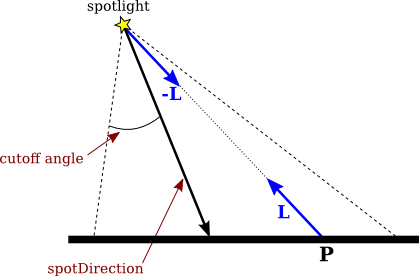
\includegraphics[height=0.45\textheight]{imagens/spotlight_3.png}
	\end{center}
\end{frame}

\begin{frame}{Nguồn sáng hình học}
	\textbf{Nguồn sáng chiếu điểm - Spot Light}\\
	\begin{center}
		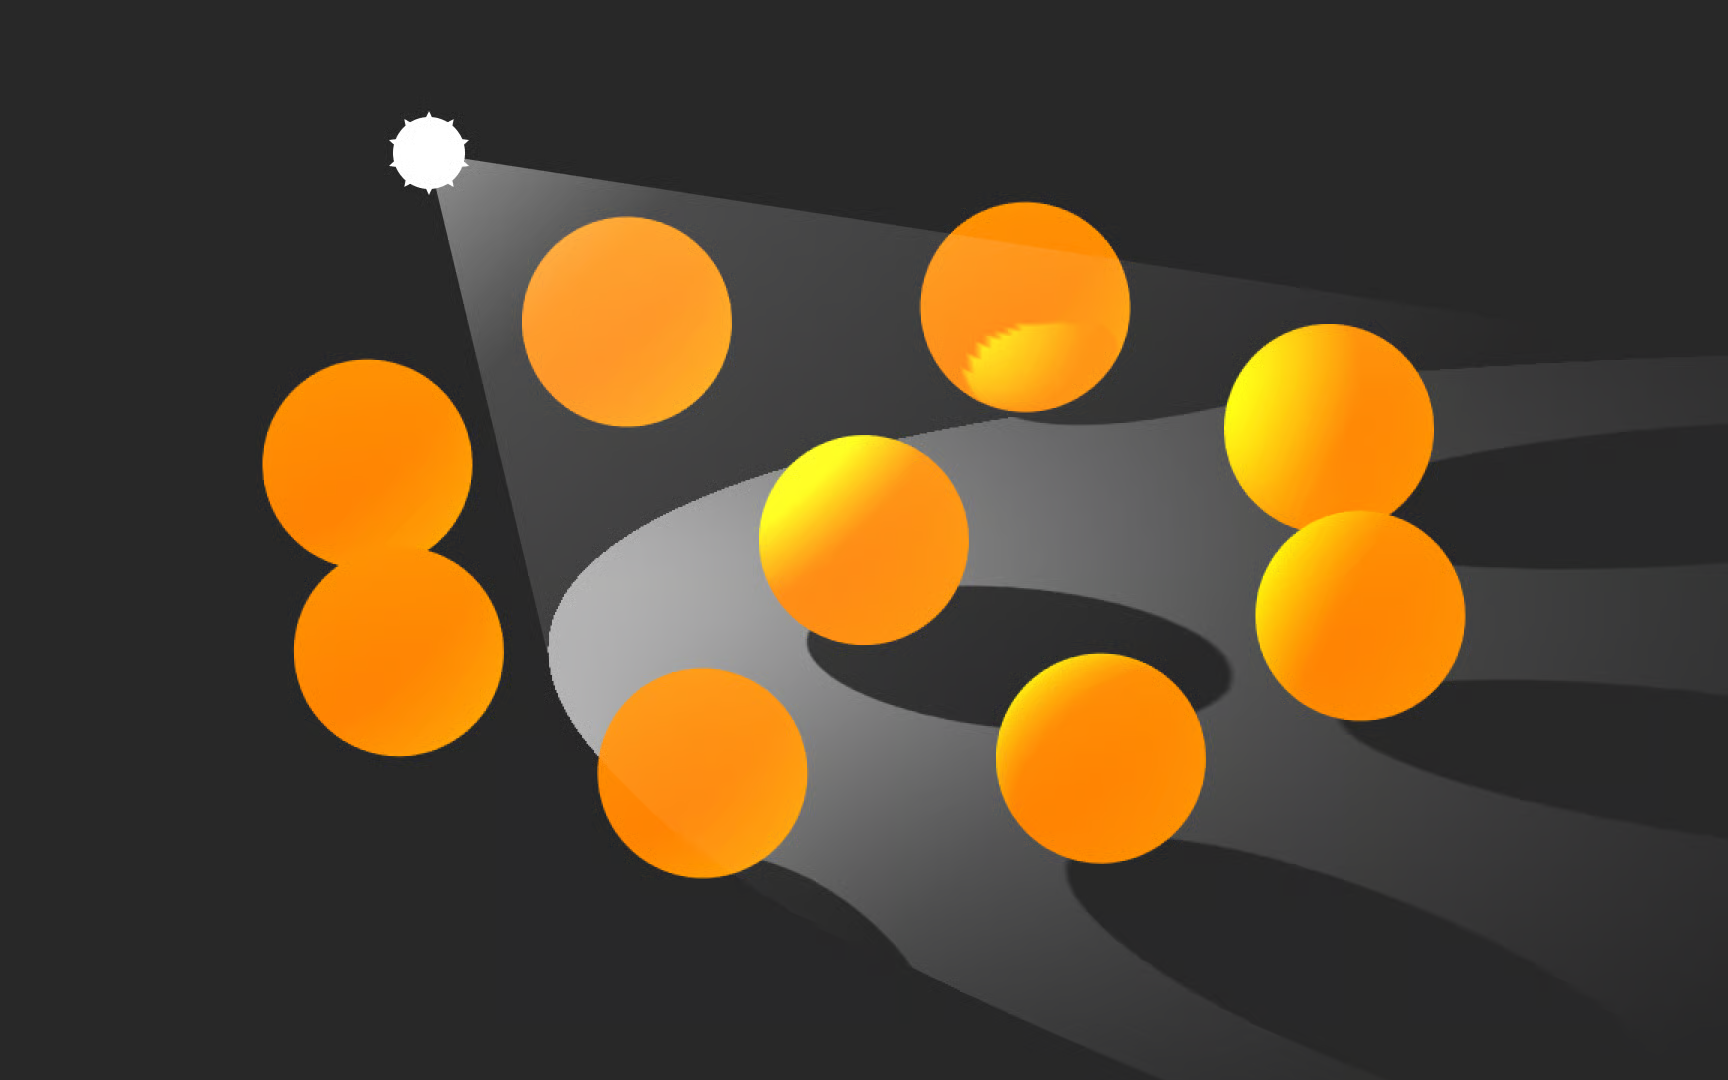
\includegraphics[height=0.45\textheight]{imagens/spotlight_1.png}
		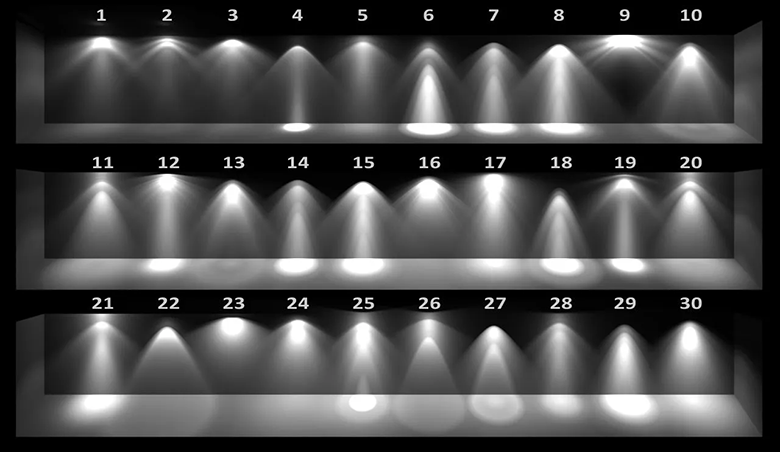
\includegraphics[height=0.45\textheight]{imagens/spotlight_2.png}
	\end{center}
\end{frame}

\begin{frame}{Mô hình chiếu sáng}
	\textbf{Nguồn sáng phi hình học - Non-Geometry Light}\\
	Nguồn sáng phi hình học là các mô hình chiếu sáng không được gán vị trí cụ thể trong cảnh, có độ sáng không đổi đến tất cả các mặt phẳng phản chiếu trong cảnh.
\end{frame}

\begin{frame}{Nguồn sáng phi hình học}
	\textbf{Nguồn sáng định hướng - Directional Light}\\
	Nguồn sáng định hướng mô phỏng một nguồn sáng ở khoảng cách vô hạn, điển hình là mặt trời. Trong mô hình này, tất cả các tia sáng được giả định là song song và có cùng cường độ tại mọi điểm trong cảnh.
	
	Đóng góp ánh sáng được tính như:
	\begin{gather*}
		I_o(x) = I_i * max(0, n \cdot l)
	\end{gather*}
	với:
	\begin{gather*}
		l = -d, \quad
		||d|| = 1
	\end{gather*}
\end{frame}

\begin{frame}{Nguồn sáng phi hình học}
	\textbf{Nguồn sáng định hướng - Directional Light}\\
	\begin{center}
		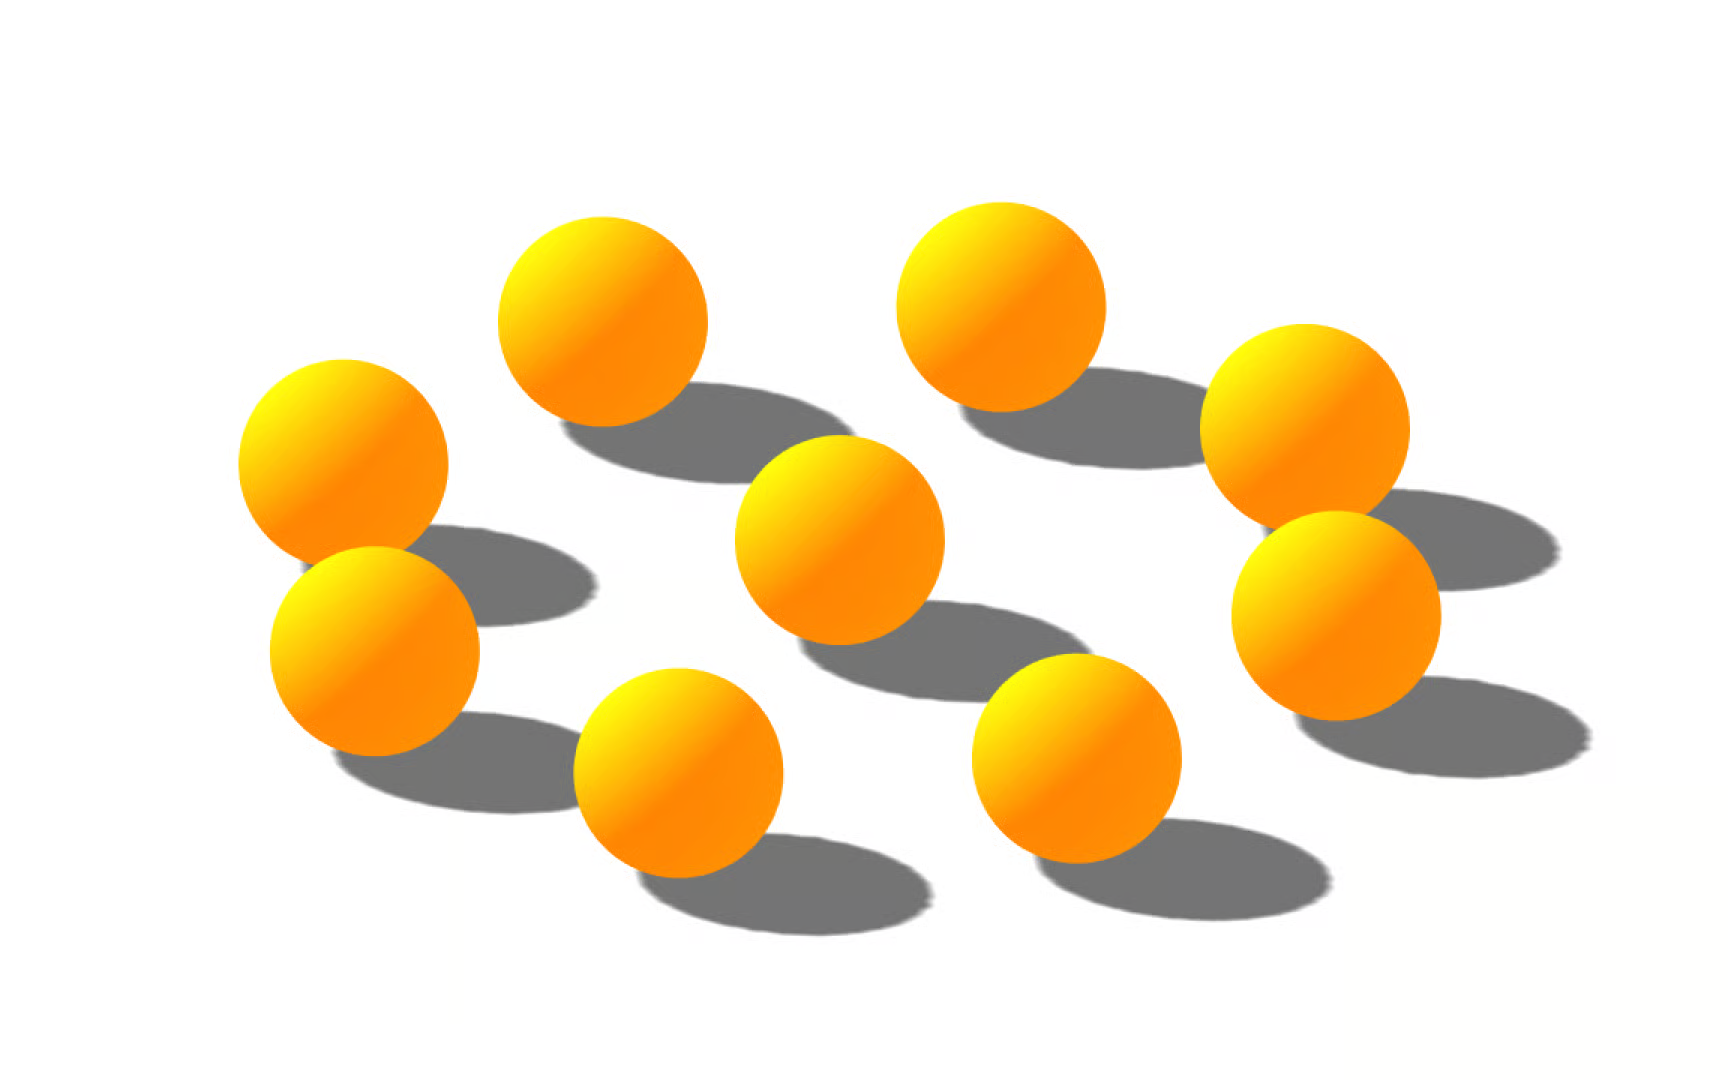
\includegraphics[height=0.35\textheight]{imagens/directionallight_1.png}
		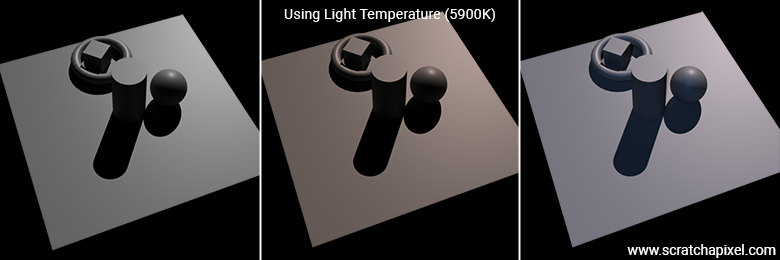
\includegraphics[height=0.35\textheight]{imagens/directionallight_2.png}
	\end{center}
\end{frame}

\begin{frame}{Nguồn sáng phi hình học}
	\begin{columns}[T]
		% --- LEFT COLUMN ---
		\begin{column}{0.4\textwidth}
			\textbf{Nguồn sáng môi trường - Ambient Light}\\
			Nguồn sáng môi trường là một mô hình xấp xỉ nhằm biểu diễn ánh sáng gián tiếp từ môi trường xung quanh. Nó cung cấp một lượng chiếu sáng đồng đều lên mọi bề mặt, không phụ thuộc vào hướng hay vị trí, nhằm tránh các vùng tối hoàn toàn trong cảnh, thường ở các bề mặt hướng ra xa khỏi nguồn sáng.
		\end{column}
		
		% --- RIGHT COLUMN ---
		\begin{column}{0.6\textwidth}
			\begin{center}
				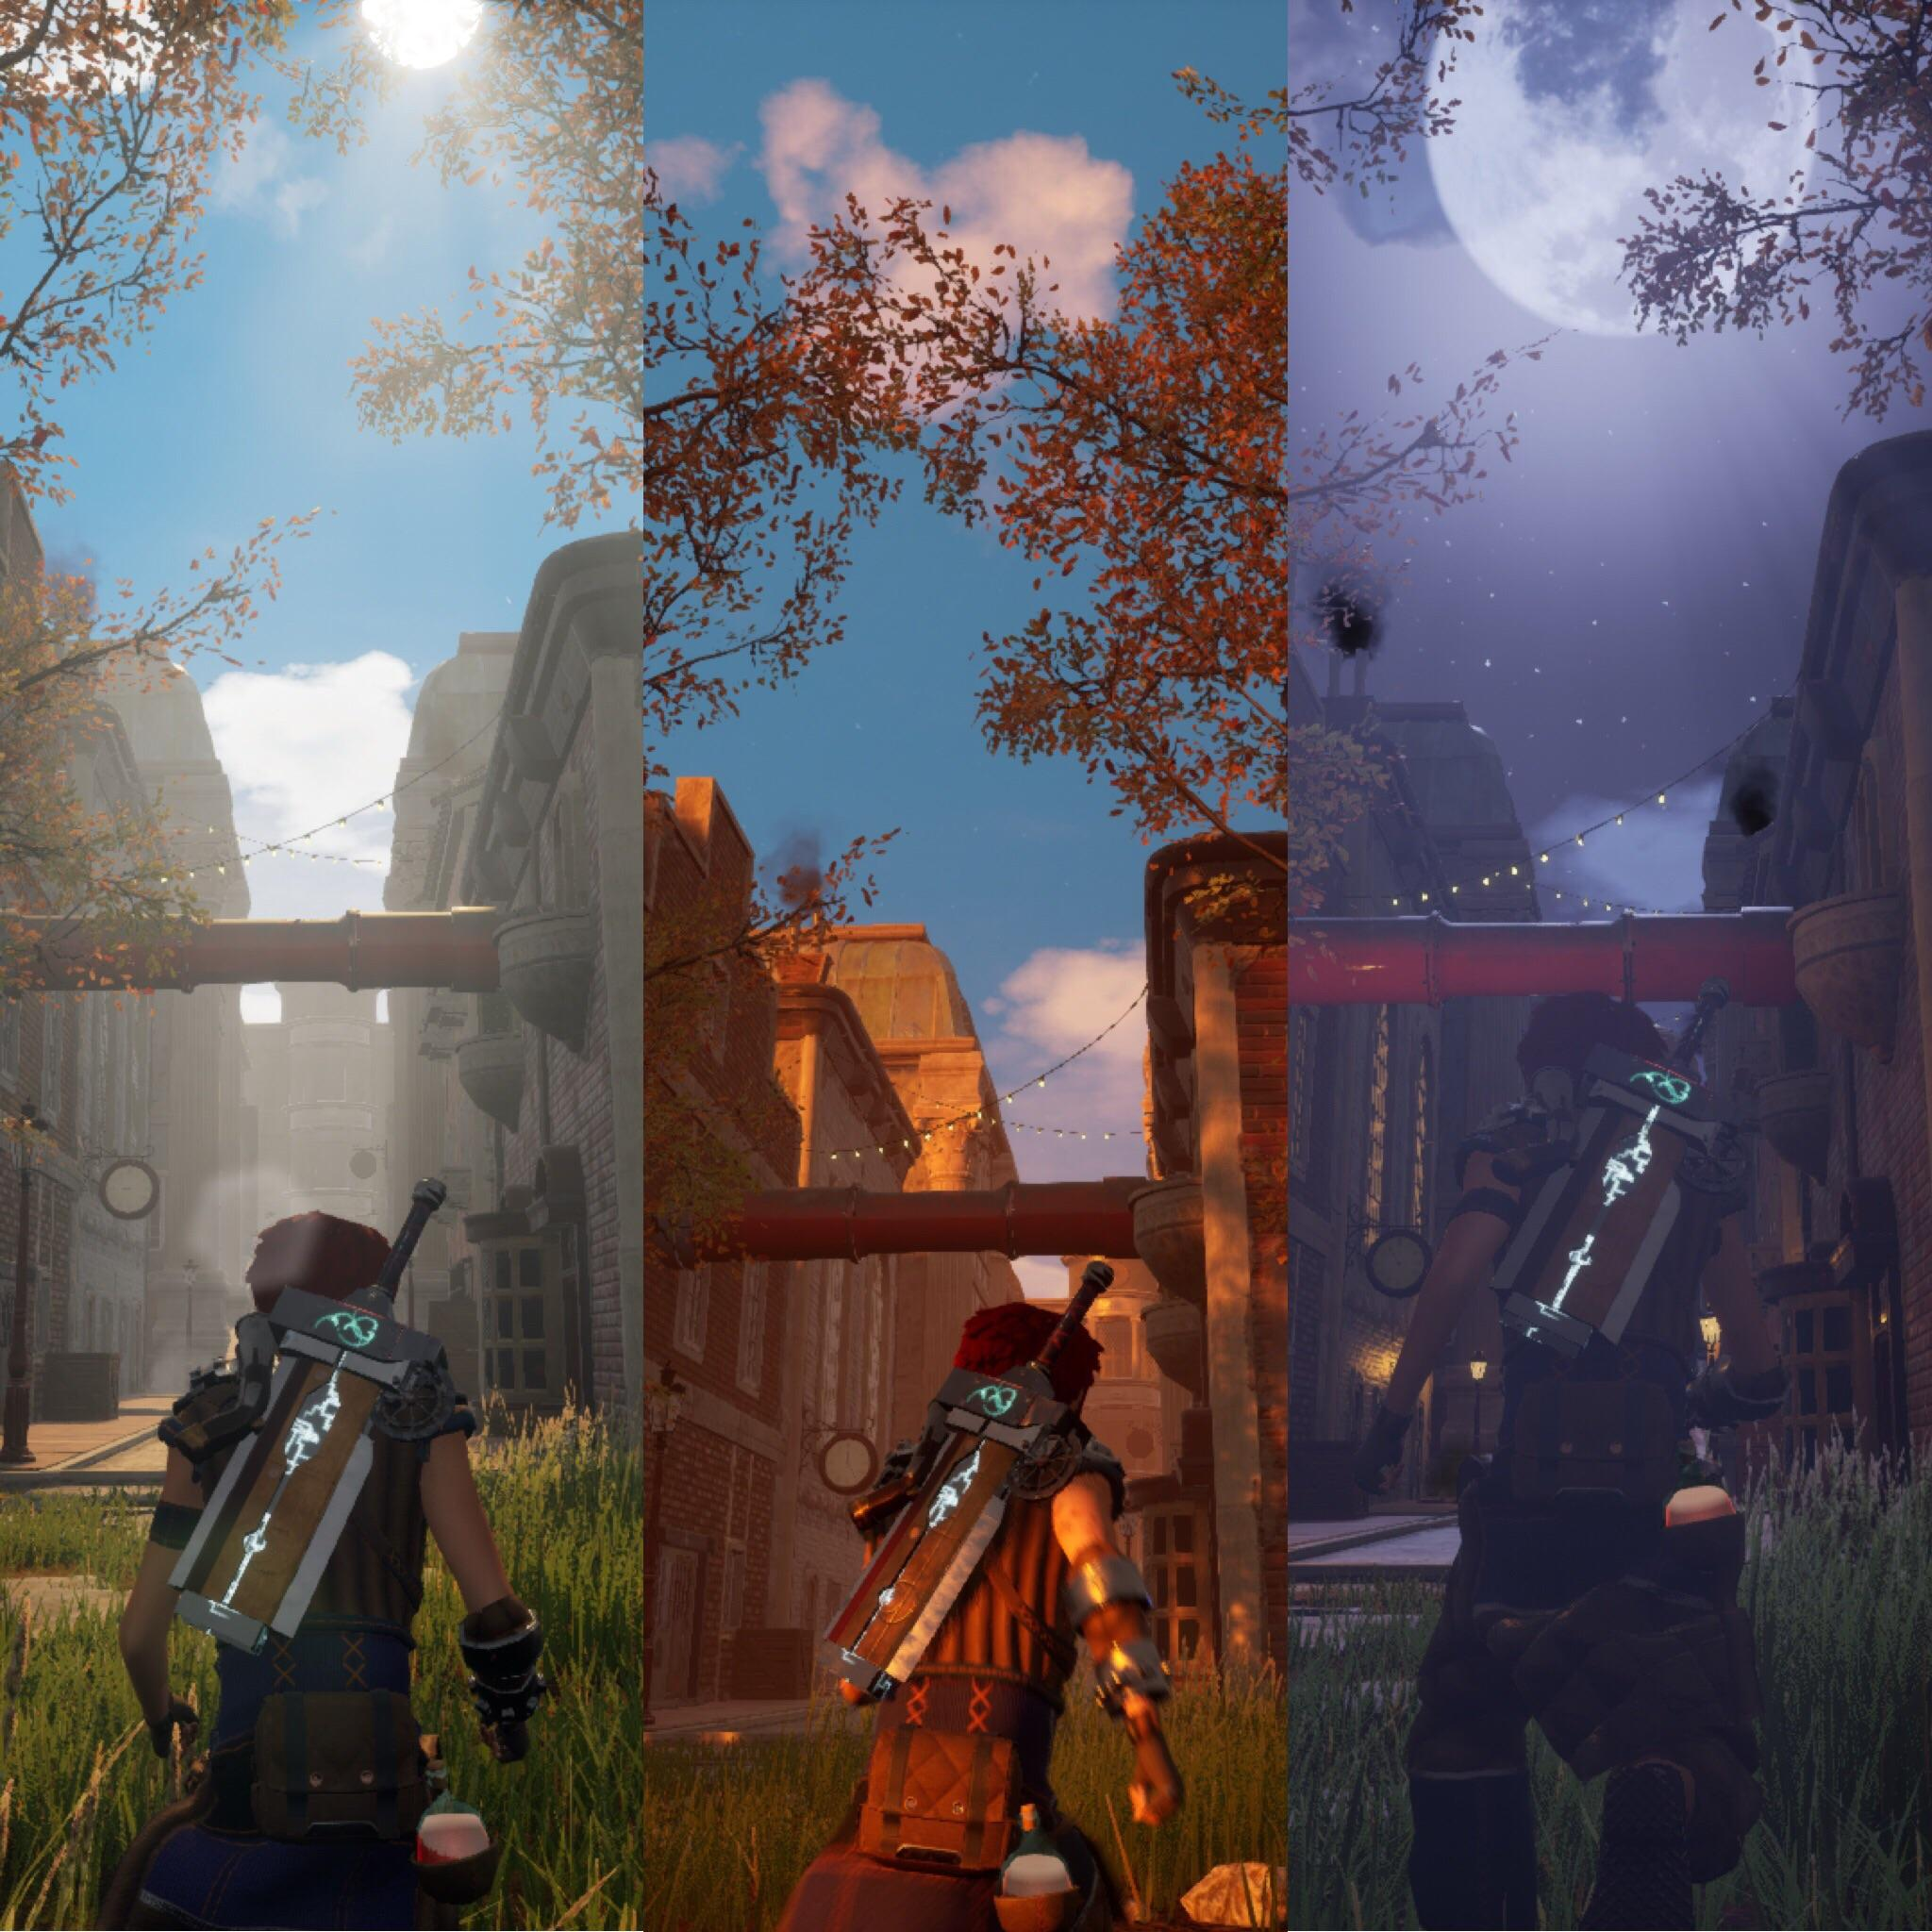
\includegraphics[width=0.7\linewidth]{imagens/ambient2.jpg}
			\end{center}
		\end{column}
	\end{columns}
	
\end{frame}

\begin{frame}{Nguồn sáng phi hình học}
	\textbf{Nguồn sáng phát xạ - Emissive Light}\\
	Nguồn sáng phát xạ mô tả các bề mặt có khả năng tự phát sáng nhưng không phải một nguồn sáng đúng nghĩa, cho phép bề mặt "phản xạ" ánh sáng ảo dù không tồn tại nguồn sáng trong cảnh, mô phỏng các vật thể tự phát sáng như đèn neon.

	\begin{center}
		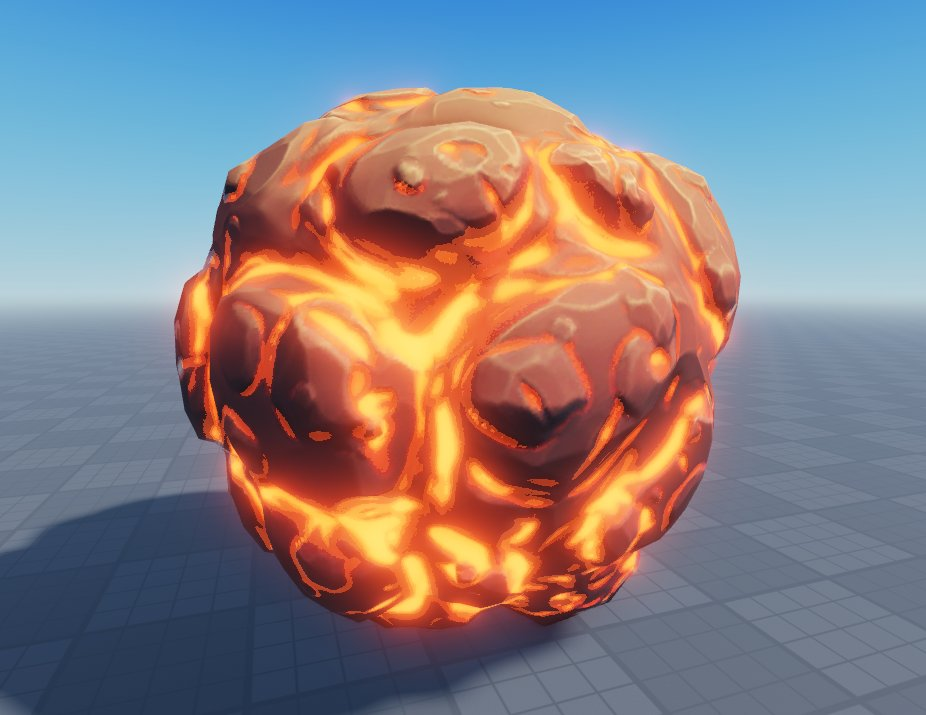
\includegraphics[height=0.35\textheight]{imagens/emission.jpg}
	\end{center}
\end{frame}

%\begin{frame}{Mô hình chiếu sáng}
%	In perfect specular ("mirror-like") reflection, an incoming ray of light is reflected from the surface intact. The reflected ray makes the same angle with the surface as the incoming ray. A viewer can see the reflected ray only if the viewer is in exactly the right position, somewhere along the path of the reflected ray. Even if the entire surface is illuminated by the light source, the viewer will only see the reflection of the light source at those points on the surface where the geometry is right. Such reflections are referred to as specular highlights. In practice, we think of a ray of light as being reflected not as a single perfect ray, but as a cone of light, which can be more or less narrow.
%	
%	
%	
%	In pure diffuse reflection, an incoming ray of light is scattered in all directions equally. A viewer would see reflected light from all points on the surface. If the incoming light arrives in parallel rays that evenly illuminate the surface, then the surface would appear to the viewer to be evenly illuminated. (If different rays strike the surface at different angles, as they would if they come from a nearby lamp or if the surface is curved, then the amount of illumination at a point depends on the angle at which the ray hits the surface at that point, but not on the angle of the line from that point to the user.)
%	
%	In pure diffuse reflection, an incoming ray of light is scattered in all directions equally. A viewer would see reflected light from all points on the surface. If the incoming light arrives in parallel rays that evenly illuminate the surface, then the surface would appear to the viewer to be evenly illuminated. (If different rays strike the surface at different angles, as they would if they come from a nearby lamp or if the surface is curved, then the amount of illumination at a point depends on the angle at which the ray hits the surface at that point, but not on the angle of the line from that point to the user.)
%\end{frame}

\subsection{Mô hình tô bóng đối tượng}
\begin{frame}{Mô hình tô bóng đối tượng}
	\begin{enumerate}
		\item Mô hình thực nghiệm
		\begin{enumerate}
			\item Flat Shading
			\item Gouraud Shading
			\item Phong Shading
			\item Blinn-Phong Shading
		\end{enumerate}
		\item Mô hình vật lý
		\begin{enumerate}
			\item Phương trình kết xuất
%			\item Phương pháp Radiosity
			\item Quy trình Physically Based Rendering - PBR
		\end{enumerate}
	\end{enumerate}
\end{frame}

\begin{frame}{Mô hình tô bóng đối tượng}
	\begin{table}[h]
		\centering
		\begin{tabular}{|l|p{10cm}|}
			\hline
			\textbf{Mô hình} & \textbf{Nguyên lý} \\ \hline
			Flat & Màu sắc tại đa giác là đồng nhất, dựa trên góc giữa pháp tuyến mặt và hướng sáng. \\ \hline
			Gouraud & Ánh sáng được tính tại các đỉnh đa giác, sau đó màu sắc được nội suy dần vào bên trong. \\ \hline
			Phong & Xấp xỉ ánh sáng phản xạ từ 3 thành phần độc lập: Môi trường (Ambient), Khuếch tán (Diffuse), và Phản xạ gương (Specular). \\ \hline
			Blinn-Phong & Biến thể của Phong, sử dụng vector trung gian (Halfway vector) để tối ưu hóa việc tính toán phản xạ gương. \\ \hline
		\end{tabular}
	\end{table}
\end{frame}

\begin{frame}{Mô hình tô bóng đối tượng}
	\begin{table}[h]
		\centering
		\begin{tabular}{|l|p{10cm}|}
			\hline
			\textbf{Mô hình} & \textbf{Nguyên lý} \\ \hline
			Rendering Equation & Ánh sáng đi ra từ điểm $x$ bằng tổng ánh sáng tự phát ra cộng với tích phân ánh sáng đi tới từ mọi hướng. \\ \hline
			Radiosity & Mô hình hóa cân bằng năng lượng nhiệt/ánh sáng cho các bề mặt phản xạ khuếch tán lý tưởng (Diffuse surfaces only). \\ \hline
			PBR & Mô phỏng tương tác ánh sáng dựa trên vật lý vi mô bề mặt (Microfacet Theory), tuân thủ bảo toàn năng lượng và hiệu ứng Fresnel. \\ \hline
		\end{tabular}
	\end{table}
\end{frame}

\begin{frame}{Mô hình tô bóng đối tượng}
	\begin{table}[h]
		\centering
		\begin{tabular}{|l|p{10cm}|}
			\hline
			\textbf{Mô hình} & \textbf{Phương pháp} \\ \hline
			Flat & Tính toán phương trình ánh sáng một lần duy nhất cho một đa giác (thường dùng pháp tuyến tại tâm). \\ \hline
			Gouraud & Tính cường độ sáng tại đỉnh, sau đó nội suy song tuyến tính màu sắc qua các pixel bên trong. \\ \hline
			Phong & Nội suy vector pháp tuyến trên từng pixel, sau đó tính toán phương trình ánh sáng cho từng pixel. \\ \hline
			Blinn-Phong & Tính tích vô hướng giữa pháp tuyến ($N$) và vector Halfway ($H$) thay vì vector phản xạ ($R$) và hướng nhìn ($V$). \\ \hline
		\end{tabular}
	\end{table}
\end{frame}

\begin{frame}{Mô hình tô bóng đối tượng}
	\begin{table}[h]
		\centering
		\begin{tabular}{|l|p{10cm}|}
			\hline
			\textbf{Mô hình} & \textbf{Phương pháp} \\ \hline
			Rendering Equation & Giải phương trình tích phân vô hạn thông qua các thuật toán xác suất như Monte Carlo, Path Tracing. \\ \hline
%			Radiosity & Chia nhỏ bề mặt thành các miếng (patches), tính hệ số hình học (Form Factors) và giải hệ phương trình tuyến tính ma trận lớn. \\ \hline
			PBR & Sử dụng các hàm phân bố phản xạ hai chiều (BRDF) phức tạp (như Cook-Torrance) kết hợp với các bản đồ (maps): Albedo, Normal, Roughness, Metalness. \\ \hline
		\end{tabular}
	\end{table}
\end{frame}

\begin{frame}{Mô hình tô bóng đối tượng}
	\begin{table}[h]
		\centering
		\begin{tabular}{|p{2cm}|p{11cm}|}
			\hline
			\textbf{Mô hình} & \textbf{Đóng góp} \\ \hline
			Flat & Chi phí tính toán cực thấp, là nền tảng sơ khai cho đồ họa 3D thời gian thực. \\ \hline
			Gouraud & Tạo ra bề mặt có cảm giác trơn mịn (smooth) với chi phí phần cứng thấp. \\ \hline
			Phong & Tạo ra điểm sáng phản xạ (highlight) rõ nét, giúp vật thể trông thực và "3D" hơn hẳn so với Gouraud. \\ \hline
			Blinn-Phong & Hiệu quả tính toán cao hơn Phong gốc; điểm sáng (highlight) trông mềm mại và tự nhiên hơn dưới nguồn sáng diện rộng. \\ \hline
			Rendering Equation & Là "Thuyết thống nhất" của đồ họa; cơ sở lý thuyết cho mọi kỹ thuật quang thực hiện đại. \\ \hline
%			Radiosity & Mô phỏng chính xác Global Illumination và bóng đổ mềm tự nhiên lần đầu tiên. \\ \hline
			PBR & Tạo ra hình ảnh nhất quán trong mọi điều kiện ánh sáng; chuẩn hóa quy trình sản xuất (workflow) giữa các phần mềm khác nhau. \\ \hline
		\end{tabular}
	\end{table}
\end{frame}

\begin{frame}{Mô hình tô bóng đối tượng}
	\begin{table}[h]
		\centering
		\begin{tabular}{|l|p{10cm}|}
			\hline
			\textbf{Mô hình} & \textbf{Hạn chế} \\ \hline
			Flat & Bề mặt vật thể bị gãy khúc (faceted), nhìn rõ các cạnh đa giác. \\ \hline
			Gouraud & Mất chi tiết phản xạ (Specular) nếu điểm sáng nằm giữa đa giác lớn; hiện tượng Mach Band. \\ \hline
			Phong & Vật thể trông giống "nhựa" (plastic look); là mô hình thực nghiệm không bảo toàn năng lượng. \\ \hline
			Blinn-Phong & Là mô hình thực nghiệm, chưa mô phỏng đúng tính chất vật lý của kim loại hay chất cách điện. \\ \hline
			Rendering Equation & Không thể giải chính xác tuyệt đối về mặt toán học; mất rất nhiều thời gian tính toán. \\ \hline
%			Radiosity & Không xử lý được vật liệu bóng/gương (Specular); tốn bộ nhớ lưu trữ; cần tính toán lại với vật thể động. \\ \hline
			PBR & Chi phí tính toán cao; đòi hỏi quy trình tạo Texture maps phức tạp và chính xác hơn. \\ \hline
		\end{tabular}
	\end{table}
\end{frame}

\subsubsection{Mô hình thực nghiệm}
\begin{frame}{Flat Shading}
	\textbf{Nguyên lý:} Với vật thể được biểu diễn bằng một lưới hình học (mesh), xem mỗi đa giác trong lưới là một mặt phẳng độc lập. Màu sắc tại đa giác là một màu đồng nhất được tính toán dựa trên góc hợp bởi vector pháp tuyến của đa giác và vector hướng tới nguồn sáng.\\
	\begin{center}
		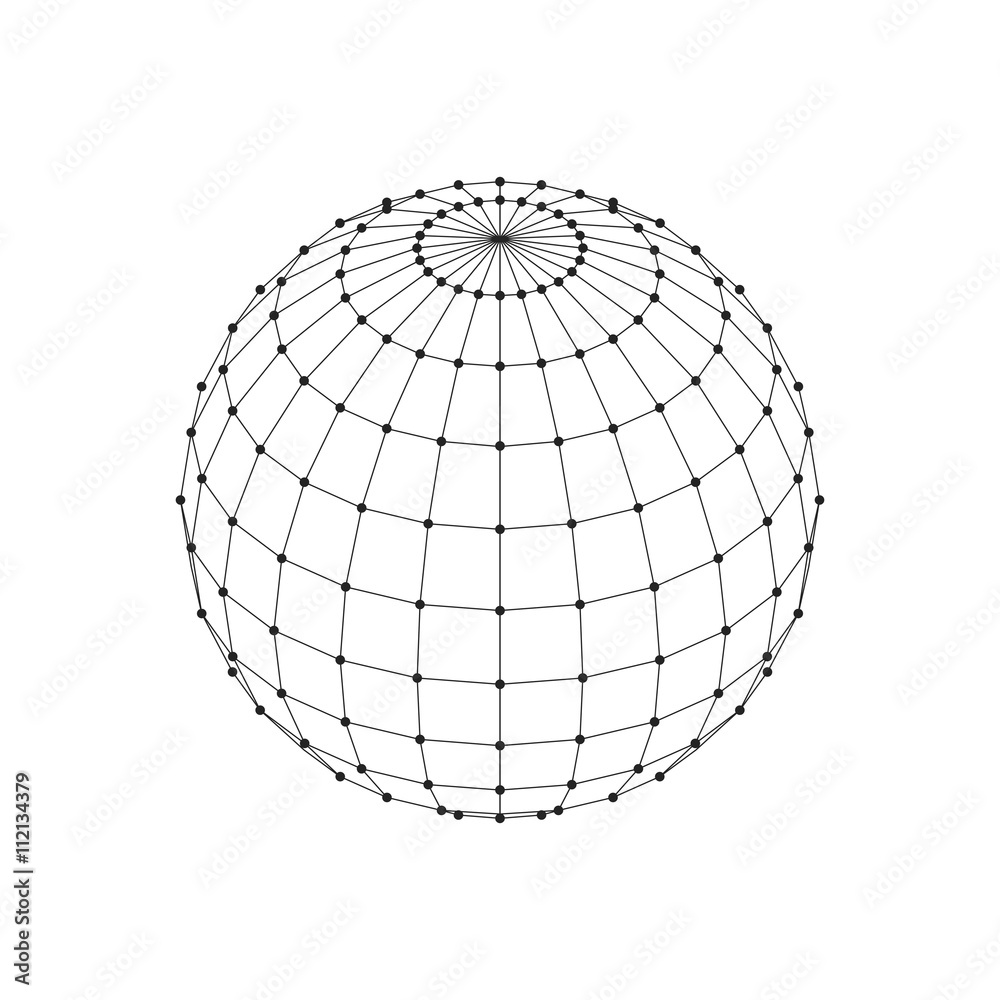
\includegraphics[height=0.3\linewidth]{imagens/sphere_1.png}
	\end{center}
\end{frame}

\begin{frame}{Flat Shading}
	\textbf{Phương pháp:}\\
	Tại mỗi đa giác, tồn tại một vector pháp tuyến duy nhất $\vec{N} = \vec{a} \times \vec{b}$, với $\vec{a}, \vec{b}$ là hai vector không song song của đa giác.\\
%	Một phép tính chiếu sáng duy nhất được thực hiện cho toàn bộ đa giác, thường chỉ sử dụng thành phần khuếch tán (diffuse) của một mô hình chiếu sáng đơn giản, tỉ lệ với góc hợp bởi vector pháp tuyến và vector hướng tới nguồn sáng.\\
\begin{center}
	\begin{math}
		I = k * I_l * max(0, \vec{N} \cdot \vec{L})
	\end{math}
\end{center}
	
%	
	Với:\\
	- $I$ là cường độ ánh sáng được tính toán.\\
	- $k$ là hệ số phản xạ, xác định mức độ hấp thụ ánh sáng của vật thể.\\
	- $I_l$ là cường độ và màu sắc nguồn sáng.\\
	- $\vec{N}$ là vector pháp tuyến đơn vị của bề mặt đa giác.\\
	- $\vec{L}$ là vector đơn vị chỉ hướng từ điểm đang xét trên bề mặt đa giác đến nguồn sáng.\\
%	Tất cả các pixel thuộc đa giác sẽ được lấp đầy bằng giá trị $I$.
\end{frame}

\begin{frame}{Flat Shading}
	\textbf{Đóng góp:} Hiệu suất tính toán của tô bóng phẳng rất cao. Vì chỉ có một phép tính chiếu sáng cho mỗi đa giác, đây là phương pháp nhanh nhất có thể, cho phép các hệ thống phần cứng sơ khai có thể kết xuất các cảnh 3D rắn trong thời gian thực.\\
	\textbf{Hạn chế:} Vì mỗi đa giác có một màu riêng biệt, các bề mặt cong được xấp xỉ bằng lưới đa giác sẽ có vẻ ngoài "gãy khúc" hoặc "khối cạnh" (faceted).
	\begin{center}
		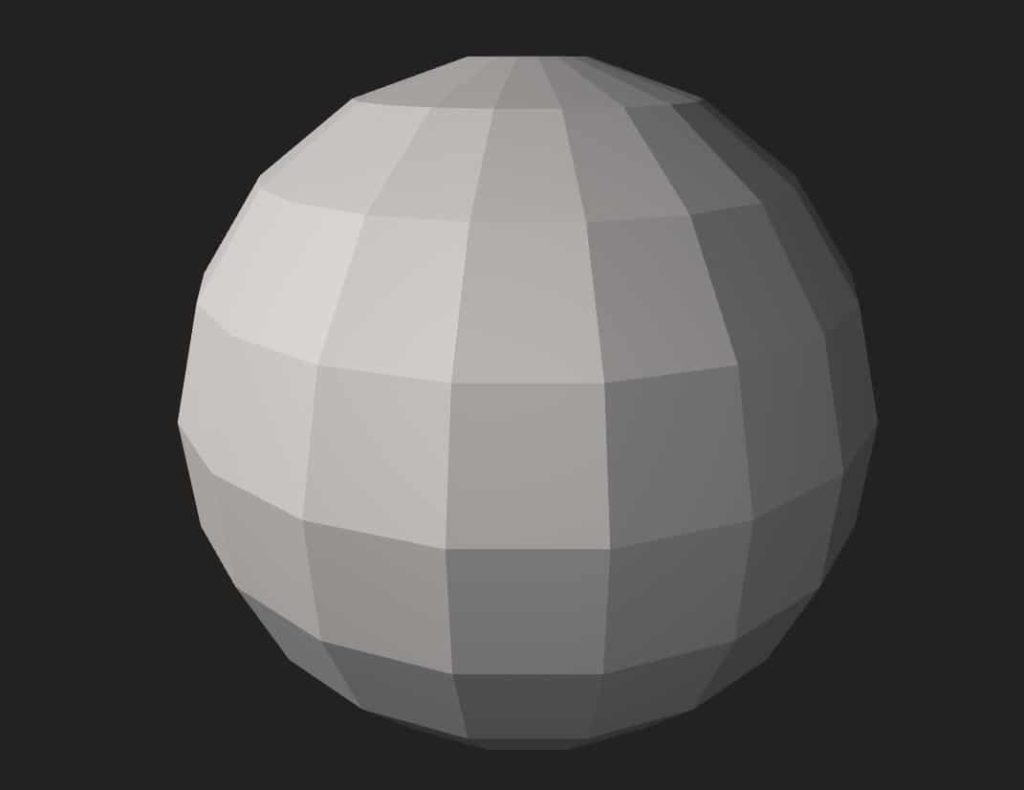
\includegraphics[height=0.25\linewidth]{imagens/sphere_2.png}
	\end{center}
\end{frame}

\begin{frame}{Gouraud Shading}
	\textbf{Nguyên lý:} Với vật thể được biểu diễn bằng một lưới hình học (mesh), xem mỗi đa giác trong lưới là một mặt phẳng độc lập. Màu sắc tại cạnh đa giác được nội suy từ các đỉnh đa giác, màu sắc tại các pixel bên trong đa giác được nội suy từ giao điểm giữa đường quét và cạnh đa giác.
	\begin{center}
		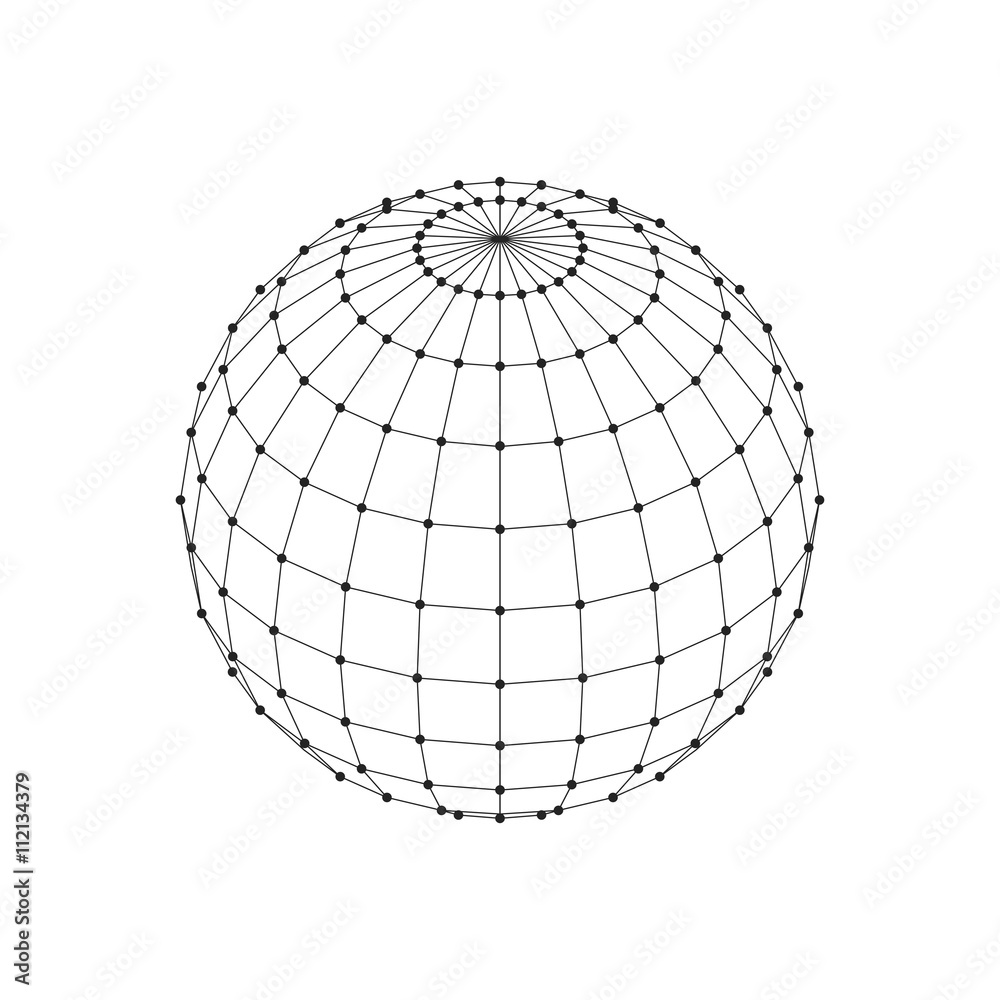
\includegraphics[height=0.3\linewidth]{imagens/sphere_1.png}
		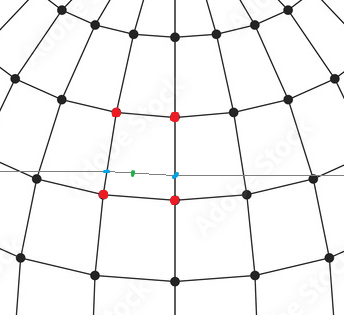
\includegraphics[height=0.3\linewidth]{imagens/sphere_1_zoom.png}
	\end{center}
\end{frame}

\begin{frame}{Gouraud Shading}
	\textbf{Phương pháp:}\\
	Tại mỗi đỉnh, tồn tại một vector pháp tuyến $\vec{N}$, được tính bằng trung bình của các pháp tuyến của các mặt chung đỉnh.
	\begin{gather*}
		\vec{N^*} = \frac{1}{m} \sum_{i=1}^{m} \vec{N_i}, \quad \quad \vec{N} = \frac{\vec{N^*}}{||\vec{N^*}||}\\
		I_v = k * I_l * max(0, \vec{N^*} \cdot \vec{L})
	\end{gather*}

	Với:\\
	- $\vec{N_i}$ là vector pháp tuyến đơn vị của bề mặt đa giác $i$.\\
	- $\vec{N}$ là vector pháp tuyến đơn vị trung bình tại đỉnh đang xét.\\
	- $\vec{L}$ là vector đơn vị chỉ hướng từ đỉnh đang xét trên bề mặt đa giác đến nguồn sáng.\\
	- $I$ là cường độ ánh sáng được tính toán.\\
	- $k$ là hệ số phản xạ, xác định mức độ hấp thụ ánh sáng của vật thể.\\
	- $I_l$ là cường độ và màu sắc nguồn sáng.\\
\end{frame}

\begin{frame}{Gouraud Shading}
	Tại mỗi dòng quét cắt qua đa giác, cường độ màu tại các giao điểm trên các cạnh của đa giác được nội suy tuyến tính từ màu của các đỉnh tương ứng.\\
	\begin{center}
		\begin{math}
			I_i = t * I_A + (1 - t) * I_B \quad t \in [0; 1]
		\end{math}
	\end{center}
%	
	Với:\\
	- $I_i$ là cường độ ánh sáng tại một điểm trên cạnh nối giữa đỉnh A và B.\\
	- $I_A, I_B$ là cường độ ánh sáng tại hai đỉnh A và B.\\
%	
	Tại mỗi pixel trên dòng quét nằm bên trong đa giác, cường độ màu được nội suy từ màu của các giao điểm trên cạnh.\\
	\begin{center}
		\begin{math}
			I_j = t * I_1 + (1 - t) * I_2 \quad t \in (0; 1)
		\end{math}
	\end{center}
%	
	Với:\\
	- $I_j$ là cường độ ánh sáng tại một điểm nằm trên dòng quét.\\
	- $I_1, I_2$ là cường độ ánh sáng tại hai giao điểm giữa dòng quét và các cạnh đa giác.
\end{frame}

\begin{frame}{Gouraud Shading}
	\begin{columns}[T]
		
		% --- LEFT COLUMN ---
		\begin{column}{0.5\textwidth}
			
			% TOP-LEFT CELL
			\begin{center}
				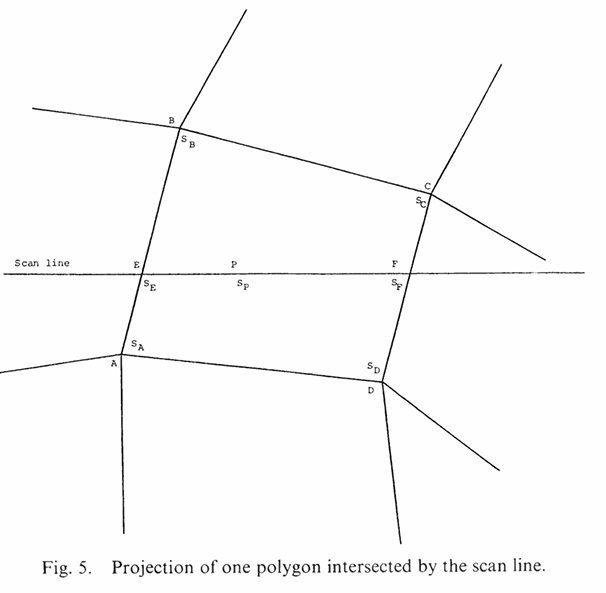
\includegraphics[height=0.55\textheight]{imagens/gouraud_1.png}
			\end{center}
			
			\vfill % Adds space between the top and bottom cells
			
			% BOTTOM-LEFT CELL
			\begin{center}
				\cite{gouraud2}
			\end{center}
			
		\end{column}
		
		% --- RIGHT COLUMN ---
		\begin{column}{0.5\textwidth}
			
			% TOP-RIGHT CELL
			\begin{center}
				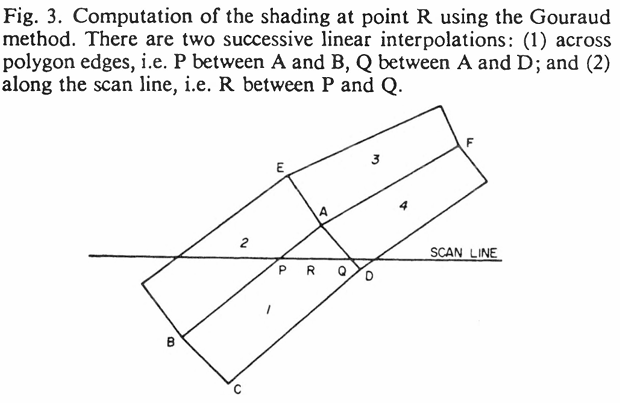
\includegraphics[height=0.55\textheight]{imagens/gouraud_2.png}
			\end{center}
			
			\vfill % Adds space between the top and bottom cells
			
			% BOTTOM-RIGHT CELL
			\begin{center}
				\cite{phong2}
			\end{center}
			
		\end{column}
		
	\end{columns}
\end{frame}

\begin{frame}{Gouraud Shading}
	\textbf{Đóng góp:} Đây là một bước đột phá lớn, cho phép các bề mặt đa giác trông mượt mà với chi phí tính toán tăng thêm không đáng kể. Mô hình Gouraud đã giải quyết hiện tượng thay đổi màu sắc đột ngột.\\
	\textbf{Hạn chế:} Vì chỉ nội suy màu, tô bóng Gouraud không thể tái tạo chính xác các hiệu ứng chiếu sáng có tần số cao, chẳng hạn như các đốm sáng phản xạ gương (specular highlights) nhỏ. Nếu một đốm sáng nằm hoàn toàn bên trong một đa giác, nó sẽ bị "nhòe" đi hoặc biến mất. Hiện tượng Mach bands cũng có thể xuất hiện.
	\begin{center}
		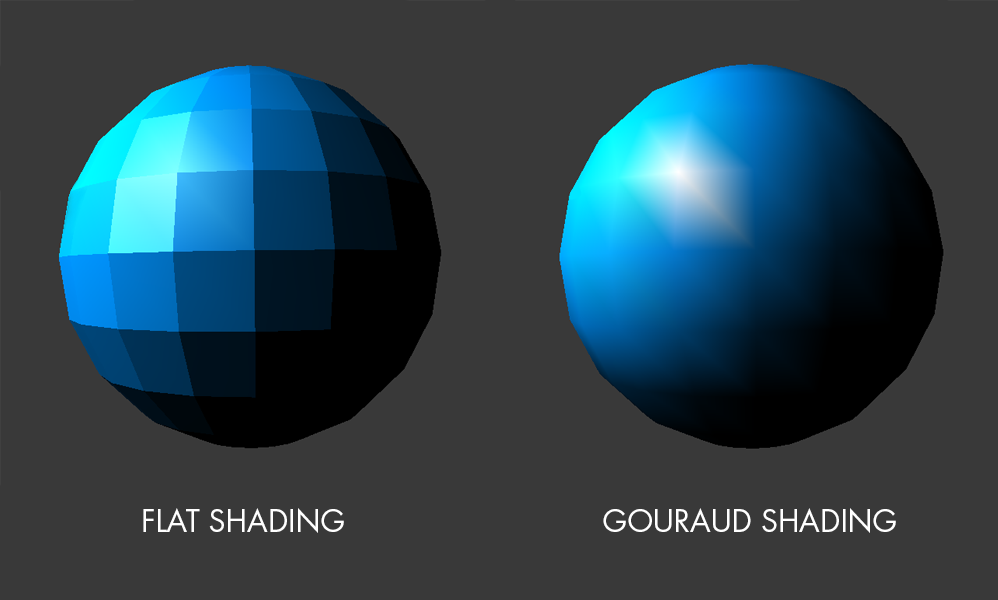
\includegraphics[height=0.2\linewidth]{imagens/sphere_3.png}
	\end{center}
\end{frame}

\begin{frame}{Phong Shading}
	\textbf{Nguyên lý:} Mô hình Phong xấp xỉ ánh sáng phản xạ từ một điểm trên bề mặt thành ba thành phần độc lập: Môi trường (Ambient), Khuếch tán (Diffuse), và Phản xạ gương (Specular).
\end{frame}

\begin{frame}{Phong Shading}
	\begin{center}
		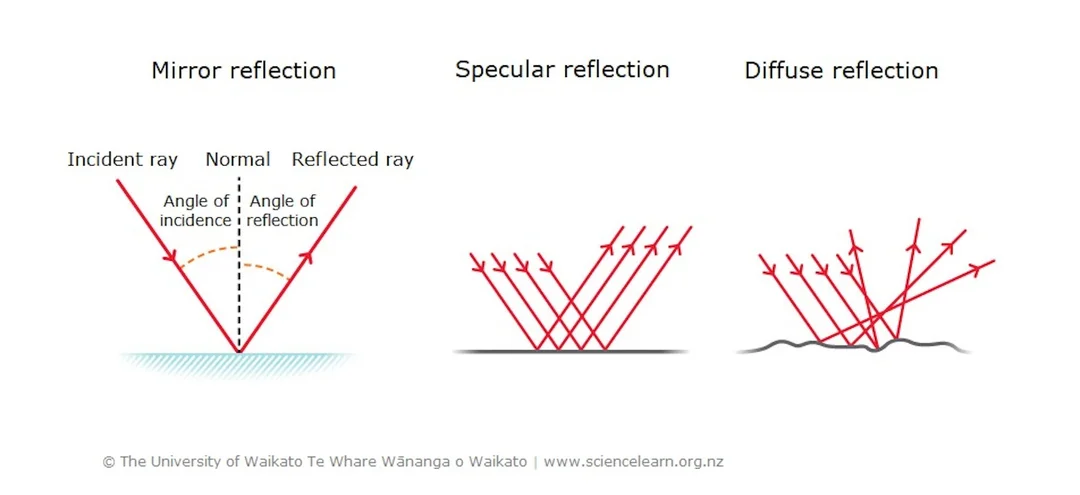
\includegraphics[width=\linewidth]{imagens/specular_vs_diffuse.png}
	\end{center}
\end{frame}

\begin{frame}{Phong Shading}
	\begin{center}
		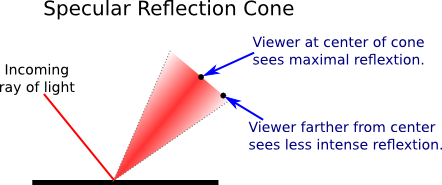
\includegraphics[width=\linewidth]{imagens/reflection-cone.png}
	\end{center}
\end{frame}

\begin{frame}{Phong Shading}
	\begin{center}
		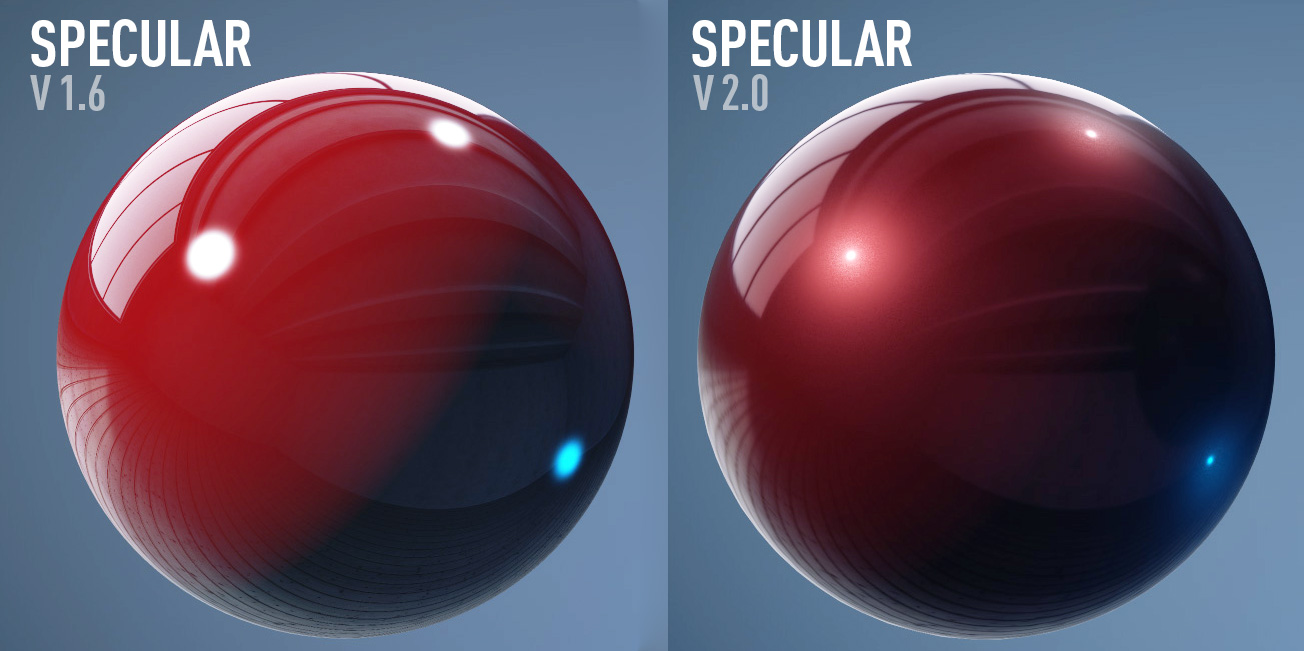
\includegraphics[width=0.9\linewidth]{imagens/specular_1.jpg}
	\end{center}
\end{frame}

\begin{frame}{Phong Shading}
	\textbf{Phương pháp:}
		\textit{Xử lý đỉnh}\\
%		Tại mỗi đỉnh, tồn tại một vector pháp tuyến $\vec{N}$, được tính bằng trung bình của các pháp tuyến của các mặt chung đỉnh.\\
		\begin{gather*}
			\vec{\hat{N}} = \frac{1}{m} \sum_{i=1}^{m} \vec{N_i}, \quad \quad \vec{N^*} = \frac{\vec{\hat{N}}}{||\vec{\hat{N}}||}\\
			I_v = k * I_l * max(0, \vec{N} \cdot \vec{L})
		\end{gather*}
		
%		
		Với:\\
		- $\vec{N_i}$ là vector pháp tuyến đơn vị của bề mặt đa giác $i$.\\
		- $\vec{N}$ là vector pháp tuyến đơn vị trung bình tại đỉnh đang xét.\\
		- $\vec{L}$ là vector đơn vị chỉ hướng từ đỉnh đang xét trên bề mặt đa giác đến nguồn sáng.\\
		- $I$ là cường độ ánh sáng được tính toán.\\
		- $k$ là hệ số phản xạ, xác định mức độ hấp thụ ánh sáng của vật thể.\\
		- $I_l$ là cường độ và màu sắc nguồn sáng.
\end{frame}
%
\begin{frame}{Phong Shading}
	\textit{Tạo lưới và nội suy (Rasterization and Interpolation)}\\
	Tạo lưới nhằm xác định tất cả các pixel trên màn hình được bao phủ bởi đa giác. Các pixel này được gọi là mảnh (fragment) trong quá trình tính toán.\\
	Vector pháp tuyến của mỗi mảnh được nội suy tuyến tính từ các vector pháp tuyến tại các đỉnh của đa giác.
\end{frame}
%
\begin{frame}{Phong Shading}
	\textit{Tính toán chiếu sáng}\\
%	Tại mỗi mảnh, mô hình Phong được áp dụng và tính toán cường độ sáng.\\
\begin{center}
	\begin{gather*}
		\vec{R^*} = 2 * (\vec{L} \cdot \vec{N}) * \vec{N} - \vec{L}, \quad \quad \quad \vec{R} = \frac{\vec{R^*}}{||\vec{R^*}||}\\
		Ambient = k_a * I_a\\
		Diffuse = k_d * I_d * max(0, \vec{N} \cdot \vec{L})\\
		Specular = k_s * I_s * max(0, \vec{R} \cdot \vec{V})^n\\
		I = Ambient + Diffuse + Specular
	\end{gather*}
\end{center}
%	
	Với:\\
	- $k_a, k_d, k_s$ là hệ số phản xạ môi trường, khuếch tán, phản xạ gương tương ứng với các thành phần ánh sáng.\\
	- $I_a, I_d, I_s$ là cường độ của các thành phần ánh sáng.\\
	- $\vec{N}$ là vector pháp tuyến đơn vị của mảnh.\\
	- $\vec{L}$ là vector đơn vị chỉ hướng từ mảnh đang xét đến nguồn sáng.\\
	- $\vec{R}$ là vector đơn vị phản xạ hướng chiếu sáng.\\
	- $\vec{V}$ là vector đơn vị từ vị trí của mảnh đến camera.
\end{frame}

\begin{frame}{Phong Shading}
	\begin{center}
		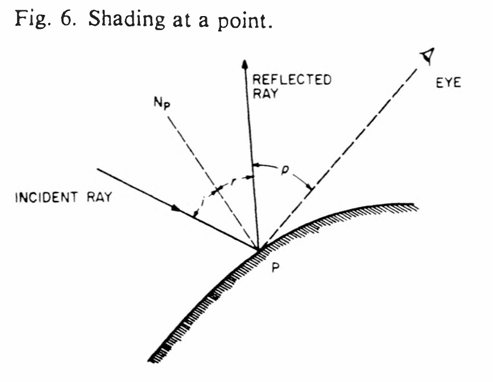
\includegraphics[height=0.4\linewidth]{imagens/phong_1.png}\\
		\cite{phong2}
	\end{center}
\end{frame}

\begin{frame}{Phong Shading}
	\textbf{Đóng góp:} Tô bóng Phong tạo ra các đốm sáng phản xạ gương mượt mà và chính xác hơn nhiều. Mô hình đã trở thành tiêu chuẩn trong nhiều thập kỷ cho cả đồ họa thời gian thực và ngoại tuyến.\\
	\textbf{Hạn chế:} Chi phí tính toán cao hơn đáng kể so với Gouraud. Mô hình vẫn mang tính thực nghiệm và không tuân thủ các nguyên tắc vật lý.
	\begin{center}
		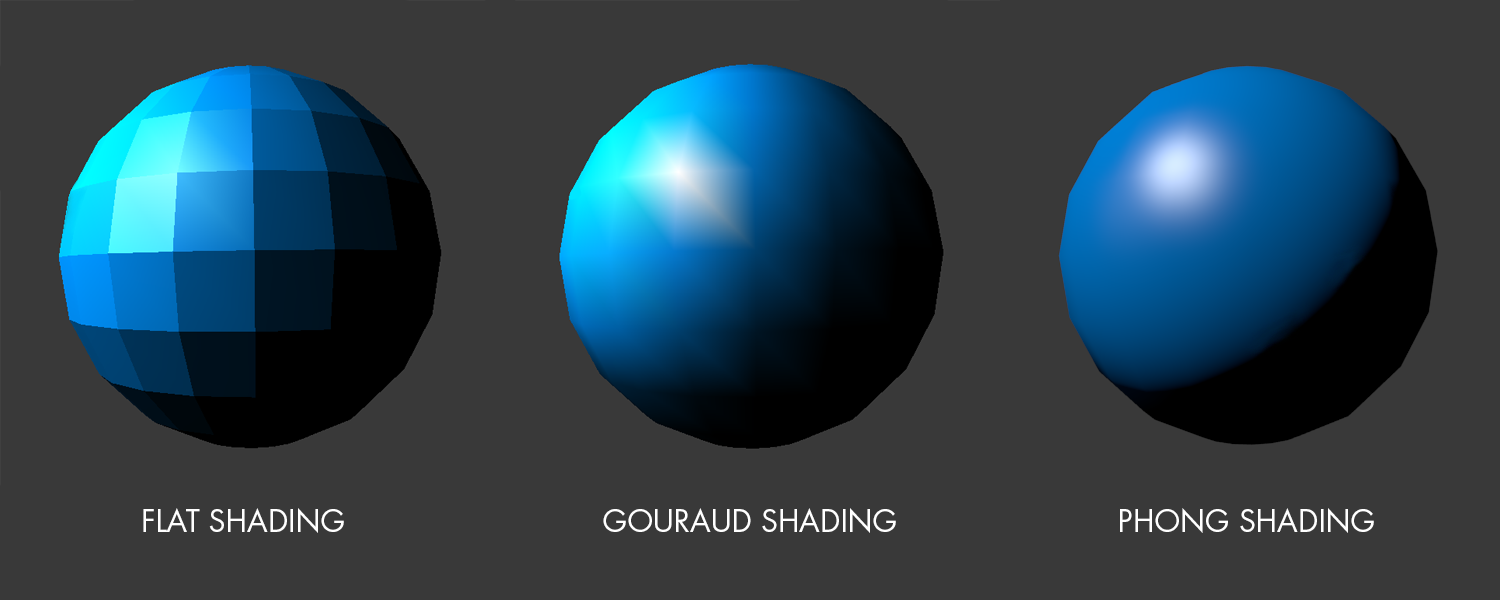
\includegraphics[height=0.3\linewidth]{imagens/sphere_4.png}
	\end{center}
\end{frame}

\begin{frame}{Blinn-Phong Shading}
	\textbf{Phương pháp:} Tương tự mô hình của Phong\\

	Tại thành phần phản xạ gương, thay thế vector phản xạ $\vec{R}$ bằng vector nửa góc (Halfway vector) $\vec{H}$.\\
	\begin{gather*}
		\vec{H} = \frac{\vec{L} + \vec{V}}{||\vec{L} + \vec{V}||}\\
		Specular = k_s * I_s * max(0, \vec{R} \cdot \vec{V})^n
	\end{gather*}
	Với:\\
	- $k_s$ là hệ số phản xạ gương tương ứng với thành phần ánh sáng.\\
	- $I_s$ là cường độ của thành phần ánh sáng.\\
	- $\vec{L}$ là vector đơn vị chỉ hướng từ mảnh đang xét đến nguồn sáng.\\
	- $\vec{R}$ là vector đơn vị phản xạ hướng chiếu sáng.\\
	- $\vec{V}$ là vector đơn vị từ vị trí của mảnh đến camera.\\
	- $\vec{H}$ là vector đơn vị nửa góc.
\end{frame}

\begin{frame}{Blinn-Phong Shading}
	\textbf{Đóng góp:} Việc tính toán $\vec{H}$ thường hiệu quả hơn $\vec{R}$. Mô hình này cũng cho kết quả trông tự nhiên hơn trong một số trường hợp. Do hiệu quả của mô hình, Blinn-Phong đã được sử dụng rộng rãi làm mô hình chiếu sáng mặc định trong các API đồ họa đời đầu như OpenGL và Direct3D.
	
	\textbf{Hạn chế:} Tương tự như mô hình Phong, đây vẫn là một mô hình thực nghiệm và không có cơ sở vật lý.
	
	\begin{center}
		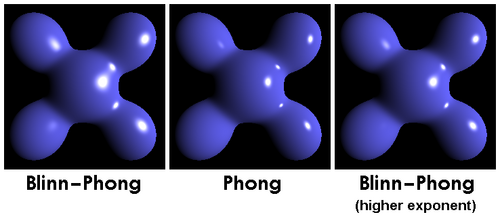
\includegraphics[height=0.3\linewidth]{imagens/blinn_phong_1.png}
	\end{center}
\end{frame}

\subsubsection{Mô hình vật lý}

\begin{frame}{Phương trình kết xuất}
	\textbf{Nguyên lý:} Phương trình Kết xuất là một biểu thức vật lý mô tả trạng thái cân bằng của bức xạ ánh sáng tại mọi điểm trong một cảnh. Nó phát biểu rằng, ánh sáng đi ra $(L_o)$ từ một điểm x theo một hướng $\omega_o$ bằng tổng của ánh sáng do chính điểm đó phát ra $(L_e)$ và tích phân của tất cả ánh sáng đi tới $(L_i)$ từ mọi hướng $\omega_i$ trên bán cầu $\Omega$ xung quanh điểm đó, được điều chỉnh bởi hàm phân bố tán xạ hai chiều (BRDF) của bề mặt\cite{render_equa1}.
\end{frame}

\begin{frame}{Phương trình kết xuất}
	\textbf{Phương pháp:}\\
	Phương trình có dạng tích phân Fredholm loại thứ hai:\\
	\begin{gather*}
			L_o(x, \omega_o) = L_e(x, \omega_o) + \int_\Omega f_r(x, \omega_i, \omega_o) * L_i(x, \omega_i)(n \cdot \omega_i) d\omega_i\\
			L_o \approx L_e + \frac{1}{N} \Sigma_{k=1}^N \frac{f_r(x, \omega_k, \omega_o) * L_i(\omega_k)(n \cdot \omega_i) d\omega_i}{p(\omega_k)}
	\end{gather*}
	\begin{center}
		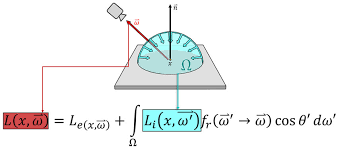
\includegraphics[width=0.5\linewidth]{imagens/rendering_equa1.png}
	\end{center}
\end{frame}

\begin{frame}{Phương trình kết xuất}
	\textbf{Đóng góp:}\\
	Cung cấp một nền tảng lý thuyết thống nhất cho tất cả các thuật toán kết xuất dựa trên vật lý.\\
	Cho phép mô phỏng một cách tự nhiên và toàn diện tất cả các hiện tượng quang học phức tạp.\\
	Là nền tảng cho hầu hết các trình kết xuất quang thực hiện đại được sử dụng trong sản xuất phim ảnh và hiệu ứng kỹ xảo.
	
	\textbf{Hạn chế:}\\
	Chi phí tính toán cực kỳ cao. Không phù hợp cho các ứng dụng thời gian thực do tốc độ hội tụ chậm.
	Bản chất ngẫu nhiên của thuật toán tạo ra nhiễu trong hình ảnh, đặc biệt là ở các khu vực có các đường đi ánh sáng phức tạp.\\
	
\end{frame}

%\begin{frame}{Phương pháp Radiosity}
%	\textbf{Nguyên lý:} Giả định tồn tại một hệ thống khép kín bao gồm các bề mặt phản xạ khuếch tán hoàn hảo (perfectly diffuse). Nó mô hình hóa sự cân bằng năng lượng ánh sáng, trong đó tổng năng lượng ánh sáng rời khỏi một bề mặt bằng tổng năng lượng do chính nó phát ra với năng lượng nó phản xạ lại từ tất cả các bề mặt khác trong cảnh. Đặc điểm quan trọng nhất là nó tính toán sự tương tác ánh sáng gián tiếp giữa các bề mặt, tạo ra các hiệu ứng như chảy máu màu (color bleeding)\cite{radiosity1}.
%	
%	\begin{center}
%		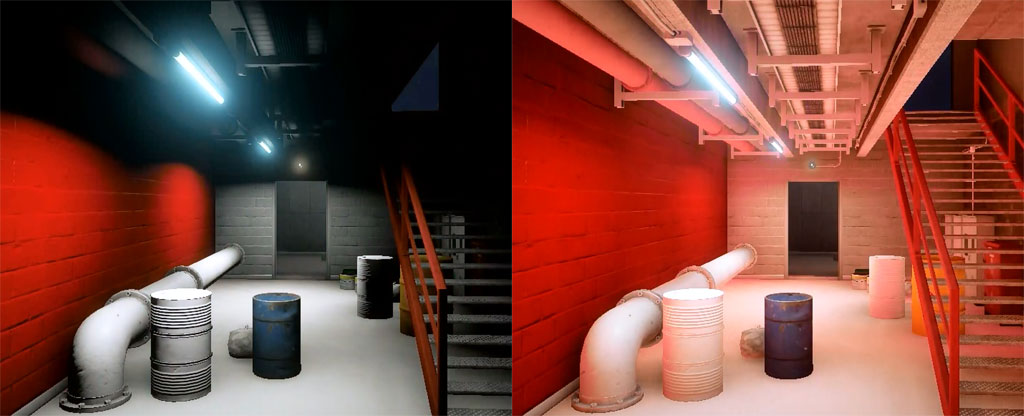
\includegraphics[height=0.25\linewidth]{imagens/radiosity_1.jpg}
%	\end{center}
%\end{frame}

%\begin{frame}{Phương pháp Radiosity}
%	\textbf{Phương pháp:}\\
%	\begin{enumerate}
%		\item Rời rạc hóa (Discretization)\\
%		Toàn bộ các bề mặt trong cảnh được chia nhỏ thành một tập hợp các ô (patches) đa giác phẳng.
%		\item Tính toán Hệ số Hình dạng (Form Factors)\\
%		Đối với mỗi cặp ô (i, j), một "hệ số hình dạng" $F_{ij}$ được tính toán. Giá trị này biểu thị phần trăm năng lượng rời khỏi ô j và chiếu tới được ô i, có tính đến khoảng cách, định hướng và sự che khuất giữa chúng.
%		\item Thiết lập hệ phương trình tuyến tính\\
%		Dựa trên nguyên lý cân bằng năng lượng, thiết lập hệ phương trình tuyến tính:\\
%		\begin{math}
%			B_i = E_i + \rho_i * \sum_{j=1}^{n}B_j * F_{ij}
%		\end{math}
%	\end{enumerate}
%	Với:\\
%	- $B_i$ là radiosity của ô $i$ (ẩn số cần tìm).\\
%	- $E_i$ là năng lượng phát ra của ô $i$.\\
%	- $\rho_i$ là hệ số phản xạ của ô $i$.
%\end{frame}

%\begin{frame}{Phương pháp Radiosity}
%	\textbf{Đóng góp:}\\
%	Đây là phương pháp đầu tiên mô phỏng thành công các hiệu ứng chiếu sáng khuếch tán gián tiếp một cách tinh tế, tạo ra các bóng đổ mềm mại và hiện tượng chảy máu màu cực kỳ chân thực, điều mà các mô hình chiếu sáng cục bộ không thể làm được\cite{radiosity1}.\\
%	Kết quả tính toán độc lập với góc nhìn. Sau khi giải hệ phương trình, các giá trị chiếu sáng được lưu lại trên các ô, cho phép người dùng di chuyển camera và kết xuất cảnh từ các góc nhìn khác nhau trong thời gian thực mà không cần tính toán lại.
%	
%	\textbf{Hạn chế:}\\
%	Mô hình giả định tất cả các bề mặt đều là phản xạ khuếch tán hoàn hảo. Do đó, Radiosity không thể mô phỏng các hiện tượng phụ thuộc vào góc nhìn như phản xạ gương, bề mặt bóng loáng, hay các vật liệu trong suốt.\\
%	Chi phí tính toán và lưu trữ rất cao, đặc biệt là ma trận hệ số hình dạng có kích thước $n * n$ với $n$ là số lượng ô.\\
%	Chỉ áp dụng được cho các cảnh tĩnh (static scenes). Bất kỳ sự thay đổi nào về hình học hoặc vật liệu đều đòi hỏi phải tính toán lại toàn bộ.
%\end{frame}

\begin{frame}{Quy trình PBR}
	\textbf{Nguyên lý:} Nguyên lý cốt lõi là tìm nghiệm cho Phương trình kết xuất bằng các mô hình vật liệu mô tả cách vật thể phản xạ ánh sáng. Những mô hình này thường được biểu diễn bởi hàm phân bố phản xạ hai chiều (Bidirectional Reflectance Distribution Function - BRDF).\\
	
	\begin{center}
		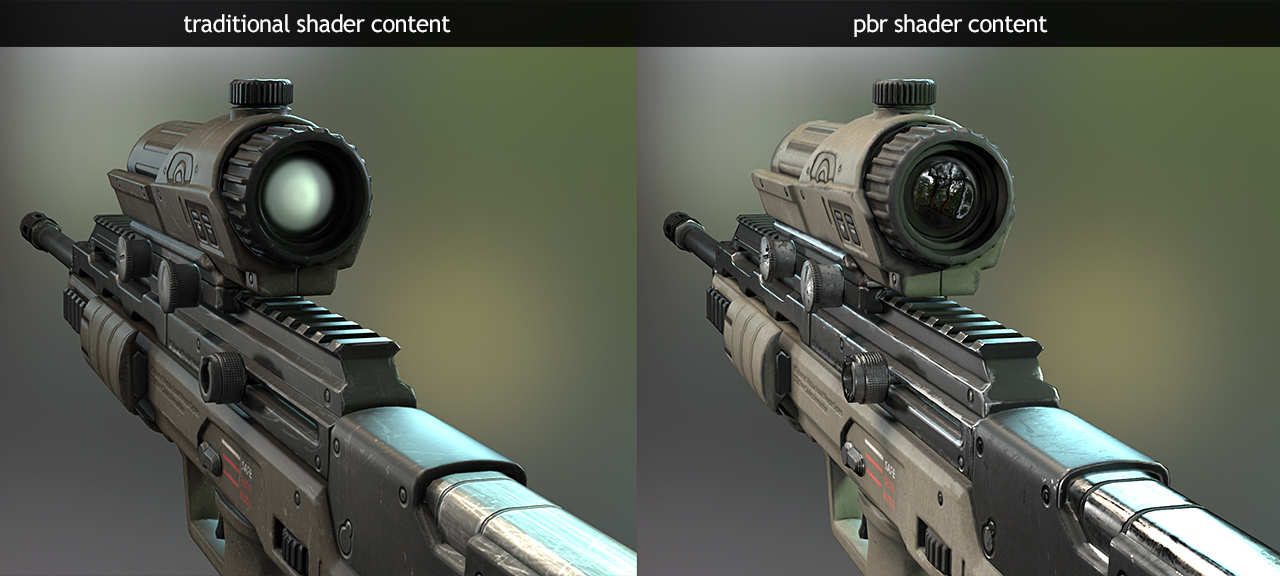
\includegraphics[height=0.25\linewidth]{imagens/pbr_1.jpg}
		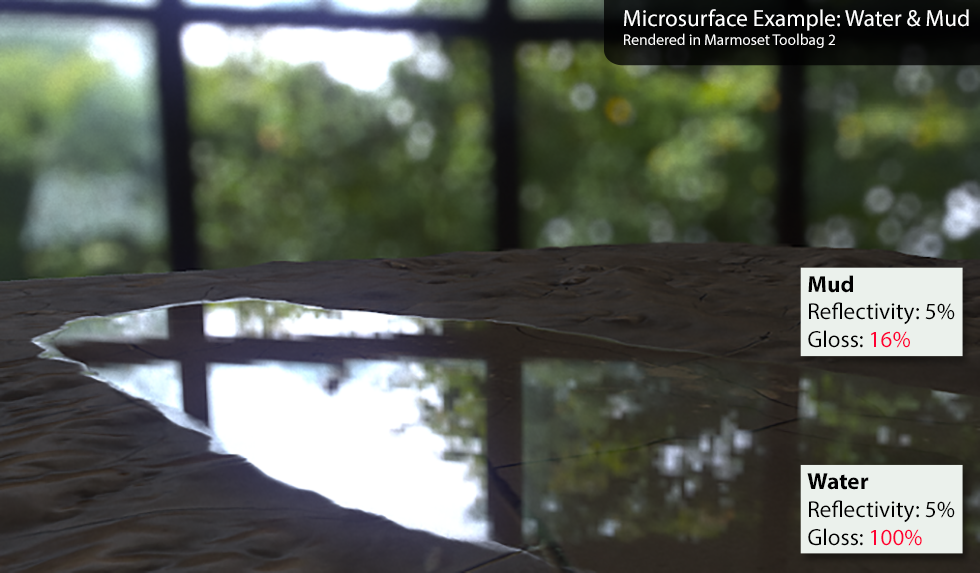
\includegraphics[height=0.25\linewidth]{imagens/pbr_2.png}
	\end{center}
\end{frame}

\begin{frame}{Quy trình PBR}
	\textbf{Đóng góp:}\\
	Tạo ra hình ảnh nhất quán trong mọi điều kiện ánh sáng; chuẩn hóa quy trình sản xuất (workflow) giữa các phần mềm khác nhau.\\
	
	\textbf{Hạn chế:}\\
	Chi phí tính toán cao; đòi hỏi quy trình tạo Texture maps phức tạp và chính xác hơn.\\
	Các mô hình PBR cần lượng lớn các tham số, các tham số này thường khó đạt được trong thực tế.\\
\end{frame}

\section{Methodology}
\begin{frame}{Phương pháp}
	Mô hình Cook-Torance dựa trên vật lý, xem xét độc lập hai thành phần: sự phân bố năng lượng quang phổ (màu sắc) và sự phân bố định hướng của ánh sáng phản xạ.\\
	Nguyên lý cốt lõi của mô hình Cook-Torrance dựa trên quang học hình học (ray theory) và mô hình vi bề mặt (microfacet model).
\end{frame}

\subsection{Lý thuyết Vi bề mặt}
\begin{frame}{Lý thuyết Vi bề mặt}
	Lý thuyết vi bề mặt giả định rằng một bề mặt thô nhám (rough surface) ở cấp độ vĩ mô thực chất được cấu tạo từ vô số các mặt phẳng gương siêu nhỏ gọi là các vi bề mặt (microfacets). Mỗi vi bề mặt này có pháp tuyến riêng và phản xạ ánh sáng theo định luật phản xạ gương lý tưởng. 
	\begin{center}
		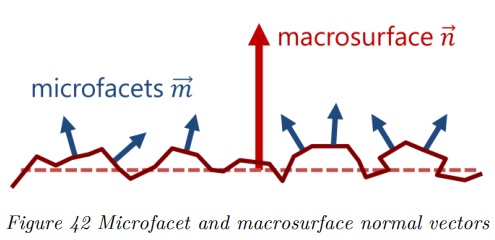
\includegraphics[width=\linewidth]{imagens/microfacet.jpg}
	\end{center}
\end{frame}

\begin{frame}{Lý thuyết Vi bề mặt}
	Chỉ những vi bề mặt nào có vector pháp tuyến hướng đúng về phía vector nửa góc (halfway vector) giữa nguồn sáng và người quan sát mới đóng góp vào thành phần phản xạ gương nhìn thấy được.
	\begin{gather*}
		\mathbf{H} = \frac{\mathbf{L} + \mathbf{V}}{||\mathbf{L} + \mathbf{V}||}
	\end{gather*}
	trong đó, $\mathbf{L}$ là vector hướng nguồn sáng đơn vị và $\mathbf{V}$ là vector hướng người quan sát đơn vị.
\end{frame}

\subsection{Các thành phần của sự phản xạ}
\begin{frame}{Các thành phần của sự phản xạ}
	Dựa trên cơ chế tương tác ánh sáng với vật liệu, mô hình Cook--Torrance chia sự phản xạ thành hai thành phần chính:
	
	\begin{enumerate}
		\item \textbf{Phản xạ gương (Specular Reflection):}\\
		Xảy ra tại bề mặt phân cách giữa không khí và vật liệu. Thành phần này mô tả ánh sáng phản xạ trực tiếp từ các vi bề mặt theo định luật phản xạ gương. Nó chịu ảnh hưởng mạnh bởi độ nhám bề mặt và chiết suất của vật liệu, đồng thời tạo ra các điểm sáng đặc trưng (specular highlights).
		
		\item \textbf{Phản xạ khuếch tán (Diffuse Reflection):}\\
		Xảy ra khi ánh sáng xâm nhập vào bên trong vật liệu, bị tán xạ nhiều lần và thoát ra ngoài theo nhiều hướng khác nhau. Thành phần này thường được giả định là khuếch tán đẳng hướng và ít phụ thuộc vào góc nhìn.
	\end{enumerate}
\end{frame}

\subsection{Hàm phân bố phản xạ hai chiều - BRDF}
\begin{frame}{Hàm phân bố phản xạ hai chiều - BRDF}
	Hàm BRDF (Bidirectional Reflectance Distribution Function) là một mô hình toán học trung tâm trong kết xuất dựa trên vật lý, dùng để mô tả cách một bề mặt phản xạ ánh sáng tại một điểm xác định. BRDF thiết lập mối quan hệ giữa ánh sáng đi tới bề mặt từ một hướng cho trước và ánh sáng được phản xạ ra khỏi bề mặt theo một hướng quan sát cụ thể. Thông qua BRDF, các đặc tính quang học của vật liệu được mã hóa một cách độc lập với hình học cảnh và nguồn sáng.
\end{frame}

\begin{frame}{Hàm phân bố phản xạ hai chiều - BRDF}
	\begin{gather*}
		f_r(p, \omega_i, \omega_o) = \frac{dL_o(p, \omega_o)}{dE_i(p, \omega_i)}
	\end{gather*}
	
	Trong đó:
	\begin{itemize}
		\item $p$ là điểm đang xét trên bề mặt.
		\item $\omega_i$ là hướng ánh sáng tới.
		\item $\omega_o$ là hướng ánh sáng phản xạ hay hướng quan sát.
		\item $dL_o$ là độ chói phản xạ theo hướng $\omega_o$.
		\item $dE_i$ là độ rọi do ánh sáng tới từ hướng $\omega_i$ gây ra.
	\end{itemize}
	
	Độ rọi vi phân có thể được viết dưới dạng:
	\begin{equation}
		dE_i = L_i(p, \omega_i) (\mathbf{N} \cdot \omega_i) \, d\omega_i
	\end{equation}
\end{frame}

\subsection{Phân rã thành các thành phần cơ bản}
\begin{frame}{Phân rã thành các thành phần cơ bản}
	Trong phần lớn các mô hình chiếu sáng và kết xuất, BRDF được phân tách thành hai thành phần chính:
	\begin{gather*}
		f_r = R_d + R_s
	\end{gather*}
	Trong đó:
	\begin{itemize}
		\item \textbf{Thành phần khuếch tán $R_d$ (Diffuse):} Mô tả sự tán xạ ánh sáng gần như đồng đều theo mọi hướng. Thành phần này thường gắn với các vật liệu điện môi, ánh sáng xâm nhập vào vật liệu, tán xạ nội tại và thoát ra ngoài. Mô hình Lambert là ví dụ đơn giản nhất của $R_d$.
		
		\item \textbf{Thành phần gương $R_s$ (Specular):} Mô tả sự phản xạ tập trung quanh hướng phản xạ gương lý tưởng. Thành phần này chịu trách nhiệm cho các vùng lóe sáng và phụ thuộc mạnh vào góc nhìn cũng như độ nhám vi mô của bề mặt. Các mô hình vi bề mặt như Cook–Torrance là những biểu diễn vật lý cho $R_s$.
	\end{itemize}
\end{frame}

\subsection{Mô hình Cook-Torrance}
\begin{frame}{Mô hình Cook-Torrance}
	\begin{equation}
		I_r = I_{ia}R_a + \sum_{l} I_{il} (\mathbf{N} \cdot \mathbf{L}_l) d\omega_{il} (sR_s + dR_d)
	\end{equation}

	\begin{itemize}
		\item $I_{ia}$ là cường độ ánh sáng môi trường, $I_{il}$ là cường độ của nguồn sáng thứ $l$.
		\item $R_a, R_s, R_d$ lần lượt là hệ số phản xạ môi trường, hệ số phản xạ gương hai chiều, hệ số phản xạ khuếch tán hai chiều.
		\item $\mathbf{N}$ là vector pháp tuyến bề mặt đơn vị,  $\mathbf{L}_l$ là vector hướng tới nguồn sáng đơn vị thứ $l$.
		\item $d\omega_{il}$ là góc khối của nguồn sáng, được xác định bởi:
		\begin{equation}
			d\omega_{il} = \frac{A}{r^2}
		\end{equation}
		với $A$ là diện tích bề mặt phát sáng và $r$ là khoảng cách tới điểm đang xét.
		\item $s$ và $d$ là trọng số của thành phần gương và khuếch tán, thỏa mãn $s + d = 1$.
	\end{itemize}
\end{frame}

\begin{frame}{Mô hình Cook-Torrance}
	\begin{equation}\label{eq:specular}
		R_s = \frac{F(\mathbf{V} \cdot \mathbf{H})}{\pi} \frac{D(\mathbf{H})\,G(\mathbf{N}, \mathbf{H}, \mathbf{V}, \mathbf{L})}{(\mathbf{N} \cdot \mathbf{L})(\mathbf{N} \cdot \mathbf{V})}
	\end{equation}
	
	Trong đó:
	
	\begin{itemize}
		\item $D(\mathbf{H})$ là hàm phân bố vi bề mặt (Facet slope distribution), biểu diễn xác suất tồn tại của các vi bề mặt có pháp tuyến cùng hướng với $\mathbf{H}$. Hàm này đặc trưng cho độ nhám bề mặt.
		\item $F(\mathbf{V}, \mathbf{H})$ là hệ số Fresnel, mô tả tỉ lệ ánh sáng bị phản xạ tại bề mặt phân cách, phụ thuộc vào góc tới và chiết suất của vật liệu.
		\item $G(\mathbf{N}, \mathbf{H}, \mathbf{V}, \mathbf{L})$ là hệ số che khuất và che bóng, mô tả hiện tượng các vi bề mặt tự che khuất hoặc che bóng lẫn nhau.
		\item $(\mathbf{N} \cdot \mathbf{L})(\mathbf{N} \cdot \mathbf{V})$ đảm bảo tính bảo toàn năng lượng và chuẩn hóa BRDF.
	\end{itemize}
\end{frame}

\begin{frame}{Mô hình Cook-Torrance}
	\begin{equation}
	D(\mathbf{H}) = \frac{1}{m^2 \cos^4 \alpha} \exp^{[-(\frac{\tan \alpha}{m})^2]}
	\end{equation}
	
	Trong đó:
	\begin{itemize}
	\item $m$ là độ dốc trung bình bình phương (root mean square slope), đại diện cho mức độ nhám vi mô của bề mặt. Giá trị $m$ nhỏ tương ứng với bề mặt bóng, tập trung nhiều vi bề mặt quanh pháp tuyến trung bình. Giá trị $m$ lớn biểu thị bề mặt thô, với các vi bề mặt phân bố rộng theo nhiều hướng khác nhau.
	\item $\alpha$ là góc giữa pháp tuyến trung bình $\mathbf{N}$ của bề mặt và vector nửa góc $\mathbf{H}$, với $\cos \alpha = \mathbf{N} \cdot \mathbf{H}$.
	\end{itemize}
\end{frame}

\begin{frame}{Mô hình Cook-Torrance}
	\begin{equation}
		G = \min \left\{
		1,\;
		\frac{2(\mathbf{N} \cdot \mathbf{H})(\mathbf{N} \cdot \mathbf{V})}{\mathbf{V} \cdot \mathbf{H}},\;
		\frac{2(\mathbf{N} \cdot \mathbf{H})(\mathbf{N} \cdot \mathbf{L})}{\mathbf{V} \cdot \mathbf{H}}
		\right\}
	\end{equation}
	\begin{equation}\label{eq:fresnel}
		F = \frac{1}{2}
		\left[
		\left( \frac{g - c}{g + c} \right)^2
		\left(
		1 +
		\left(
		\frac{c(g + c) - 1}{c(g - c) + 1}
		\right)^2
		\right)
		\right]
	\end{equation}
	Trong đó:
	\begin{itemize}
		\item $c = \cos \theta = \mathbf{V} \cdot \mathbf{H}$.
		\item $g^2 = n^2 + c^2 - 1$.
	\end{itemize}
\end{frame}

\section{Ứng dụng}
\begin{frame}{Ứng dụng}
	\begin{itemize}
		\item \textbf{Mô phỏng Nhựa (Plastics):} Sử dụng thành phần gương màu trắng (do $F$ phẳng theo bước sóng) và thành phần khuếch tán có màu. Điều này tái tạo chính xác hiệu ứng "bóng loáng" của nhựa màu.
		\item \textbf{Mô phỏng Kim loại (Metals):} Loại bỏ thành phần khuếch tán ($d \approx 0$). Thành phần gương mang màu sắc của vật liệu (ví dụ: Đồng) và thay đổi màu nhẹ khi góc nhìn chuyển sang góc nghiêng (do sự thay đổi của $F$).
	\end{itemize}
\end{frame}

\begin{frame}{Ứng dụng}
	\begin{center}
		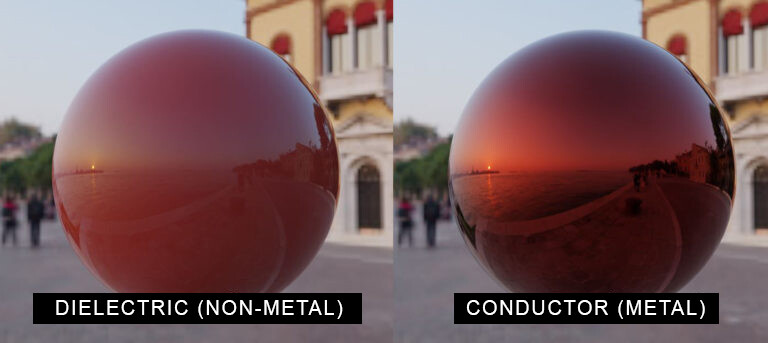
\includegraphics[width=\linewidth]{imagens/ball4.jpg}
	\end{center}
\end{frame}

\section{Implementation \& Experiment}
\begin{frame}{Cài đặt}
	\begin{itemize}
		\item OpenGL 3.3: Một hệ thống đặc tả dùng để lập trình 2D và 3D. OpenGL cung cấp tập các hàm chuẩn để giao tiếp với GPU, cho phép lập trình viên điều khiển pipeline đồ họa, viết shader, và quản lý tài nguyên như buffer, texture và framebuffer.
		\item GLFW: Thư viện hỗ trợ tạo cửa sổ và xử lý tương tác cho các ứng dụng OpenGL. GLFW chịu trách nhiệm quản lý cửa sổ, ngữ cảnh OpenGL (OpenGL context), cũng như xử lý các sự kiện bàn phím, chuột và thời gian.
		\item GLAD: Thư viện hỗ trợ nạp các con trỏ hàm OpenGL, giúp chương trình tương tác với driver của card đồ họa để sử dụng các tính năng OpenGL hiện đại.
		\item GLM: Thư viện toán học cho đồ họa máy tính, được thiết kế theo chuẩn của GLSL. GLM cung cấp các kiểu dữ liệu và phép toán cho vector, ma trận và các phép biến đổi hình học thường dùng trong đồ họa 3D.
	\end{itemize}
\end{frame}

\begin{frame}{Cài đặt}
	\begin{itemize}
		\item Assimp: Thư viện nhập mô hình 3D đa định dạng cho các ứng dụng đồ họa. Assimp hỗ trợ đọc nhiều định dạng mô hình phổ biến như OBJ, FBX, COLLADA và glTF, đồng thời chuyển đổi chúng về một cấu trúc dữ liệu trung gian thống nhất, bao gồm lưới (mesh), vật liệu (material), texture và hệ phân cấp nút (scene graph).
		\item Dear ImGui: Thư viện giao diện người dùng cho các ứng dụng đồ họa thời gian thực, cho phép xây dựng nhanh các thành phần giao diện.
	\end{itemize}
\end{frame}

\begin{frame}{Cài đặt}
	\textbf{Các chức năng chính}
	
	Hệ thống cung cấp một môi trường tương tác với các chức năng:
	\begin{enumerate}
		\item \textbf{Quản lý Vật thể:} Cho phép thêm và thao tác với các vật thể cơ bản (khối lập phương, cầu, kim tự tháp, khối trụ...) hoặc các mô hình phức tạp được tải từ bên ngoài.
		
		\item \textbf{Hệ thống Ánh sáng:} Hỗ trợ khởi tạo và tùy chỉnh ba loại nguồn sáng cơ bản:
		\begin{itemize}
			\item \textit{Directional Light:} Ánh sáng định hướng (mô phỏng mặt trời).
			
			\item \textit{Point Light:} Ánh sáng điểm (mô phỏng bóng đèn).
			
			\item \textit{Spot Light:} Ánh sáng chiếu điểm (mô phỏng đèn pin/đèn sân khấu).
		\end{itemize}
		
		\item \textbf{Chuyển đổi Mô hình Chiếu sáng:} Tính năng cốt lõi cho phép chuyển đổi tức thời giữa các shader: Phong, Blinn-Phong, Gouraud và Cook-Torrance để so sánh trực quan.
		
		\item \textbf{Chế độ Hiển thị:} Hỗ trợ các chế độ render khác nhau như khung dây (wireframe), điểm (point) và tô đặc (surface/fill).
	\end{enumerate}
\end{frame}
	
\begin{frame}{Cài đặt}
	\textbf{Kiến trúc Đối tượng}
	
	\begin{description}
		\item[Camera:] Quản lý ma trận quan sát (View Matrix) và ma trận chiếu (Projection Matrix), cho phép người dùng tự do di chuyển góc nhìn trong không gian 3D.
		\item[Light:] Lớp trừu tượng hóa các nguồn sáng, lưu trữ các thuộc tính như vị trí, hướng, màu sắc, và các hệ số suy giảm (attenuation).
		\item[Mesh \& Model:] Wrapper bao quanh thư viện Assimp, chịu trách nhiệm tải dữ liệu đỉnh (vertices), pháp tuyến (normals), và tọa độ vân (texture coordinates) từ file `.obj` và khởi tạo các bộ đệm OpenGL (VAO, VBO, EBO).
		\item[Object:] Quản lý các vật thể hình học cơ bản (Primitive shapes) như hình cầu, hình trụ. Lớp này chứa các phương thức vẽ (draw) và thiết lập thuộc tính vật liệu.
		\item[Shader:] Quản lý việc biên dịch, liên kết các shader program và truyền tải dữ liệu (uniforms) từ CPU sang GPU để tính toán ánh sáng.
	\end{description}
\end{frame}

\begin{frame}{Cài đặt}
	\textbf{Kiến trúc Đối tượng}
	\begin{description}
		\item[Shader:] Quản lý việc biên dịch, liên kết các shader program và truyền tải dữ liệu (uniforms) từ CPU sang GPU để tính toán ánh sáng.
		\item[ControlCollapse:] Lớp quản lý logic giao diện người dùng (UI Manager). Đây là cầu nối giữa ImGui và các đối tượng trong cảnh, giúp đơn giản hóa việc điều chỉnh vị trí, màu sắc, texture và các thông số vật lý (như độ nhám, chỉ số khúc xạ) thông qua các thanh trượt và menu.
		\item[Axis:] Đối tượng tiện ích hỗ trợ vẽ trục tọa độ và lưới nền (grid), giúp định vị không gian dễ dàng hơn.
	\end{description}
\end{frame}

\begin{frame}{Cài đặt}
	\textbf{Hệ thống Shader}
	\begin{itemize}
		\item \textbf{Lighting Shaders (Phong, BlinnPhong, Gouraud, CookTorrance):} Các shader chính thực hiện thuật toán tô bóng tương ứng. Riêng shader CookTorrance được cài đặt đầy đủ các công thức tính toán $D, F, G$ như đã trình bày ở phần lý thuyết.
		
		\item \textbf{Depth Shader:} Shader đặc biệt dùng để render cảnh từ góc nhìn của nguồn sáng vào một bộ đệm độ sâu (depth buffer), phục vụ cho kỹ thuật tạo bóng đổ (Shadow Mapping).
		
		\item \textbf{Axis Shader:} Shader đơn giản để vẽ các đường trục và lưới hỗ trợ.
	\end{itemize}
\end{frame}

\begin{frame}{Cài đặt}
	\textbf{Luồng hoạt động của Chương trình}
	
	\begin{itemize}
		\item \textbf{Khởi tạo (Initialization):} 
		Thiết lập ngữ cảnh OpenGL và ImGui. Cấu hình các trạng thái toàn cục (như kiểm tra độ sâu - depth test, loại bỏ mặt - cull face) giúp tối ưu hoá quá trình tính toán shader. Khởi tạo camera, ánh sáng mặc định, tải shader và các mô hình vật thể vào bộ nhớ.
		
		\item \textbf{Vòng lặp chính (Main Loop):}
		\begin{itemize}
			\item \textit{Xử lý Input:} Nhận tín hiệu từ chuột/bàn phím để di chuyển camera.
			
			\item \textit{Tạo giao diện ImGui:} Vẽ các menu điều khiển và cập nhật giá trị biến dựa trên tương tác người dùng.
			
			\item \textit{Cập nhật Uniforms:} Truyền các thông số mới (vị trí đèn, độ nhám vật liệu, ma trận biến đổi) vào shader.
		\end{itemize}
	\end{itemize}
\end{frame}

\begin{frame}{Cài đặt}
	\textbf{Luồng hoạt động của Chương trình}
	
	\begin{itemize}
		\begin{itemize}
			\item \textit{Bước 1 - Shadow Pass:} Render cảnh từ vị trí nguồn sáng để tạo Shadow Map (bản đồ bóng).
			
			\item \textit{Bước 2 - Render Scene:} Render cảnh từ góc nhìn camera sử dụng shader ánh sáng được chọn, kết hợp với Shadow Map để tính toán bóng đổ.
			
			\item \textit{Swap Buffers:} Hiển thị khung hình mới lên màn hình.
		\end{itemize}
		
		\item \textbf{Kết thúc (Termination):} Giải phóng tài nguyên bộ nhớ (VAO, VBO, textures) và hủy ngữ cảnh GLFW/ImGui.
	\end{itemize}
\end{frame}

\begin{frame}{Các hàm và đối tượng bộ đệm được sử dụng trong OpenGL}
	\begin{itemize}
		\item \textbf{VAO (Vertex Array Object):} Đối tượng bao đóng cấu hình. Nó không chứa dữ liệu thực mà lưu trữ trạng thái về cách OpenGL nên đọc dữ liệu từ VBO (ví dụ: 3 số đầu là vị trí, 3 số sau là pháp tuyến). Hàm liên quan: \texttt{glGenVertexArrays}, \texttt{glBindVertexArray}.
		\item \textbf{VBO (Vertex Buffer Object):} Bộ đệm chứa dữ liệu thô (raw data) của các đỉnh (vertices). Dữ liệu vị trí, pháp tuyến, và tọa độ texture được gửi từ RAM sang VRAM thông qua đối tượng này. Hàm liên quan: \texttt{glGenBuffers}, \texttt{glBufferData}.
		\item \textbf{EBO (Element Buffer Object):} Bộ đệm lưu trữ danh sách các chỉ số (indices). Nó cho phép OpenGL tái sử dụng các đỉnh trùng lặp (ví dụ: các đỉnh chung của hai tam giác kề nhau), giúp tiết kiệm bộ nhớ và tối ưu hóa hiệu năng.
		\item \textbf{FBO (Framebuffer Object):} Bộ đệm khung hình tùy chỉnh. Thay vì vẽ trực tiếp lên màn hình, chương trình vẽ vào FBO để thực hiện các kỹ thuật xử lý hậu kỳ hoặc tính toán trung gian.
	\end{itemize}
\end{frame}

\begin{frame}{Các hàm và đối tượng bộ đệm được sử dụng trong OpenGL}
	\begin{itemize}
		\item \texttt{glGenTextures} và \texttt{glBindTexture}: Tạo ID và kích hoạt đối tượng texture hiện hành.
		\item \texttt{glTexImage2D}: Chuyển dữ liệu điểm ảnh (pixel data) từ CPU sang GPU để tạo thành texture 2D.
		\item \texttt{glTexParameteri}: Thiết lập các tham số hiển thị, ví dụ như chế độ lặp lại (GL\_REPEAT) hoặc bộ lọc tuyến tính (GL\_LINEAR) khi phóng to/thu nhỏ texture.
		\item \texttt{glActiveTexture}: Kích hoạt các đơn vị texture (Texture Units -\\ GL\_TEXTURE0, GL\_TEXTURE1...) để shader có thể đọc nhiều texture cùng lúc (ví dụ: vừa đọc Albedo map, vừa đọc Shadow map).
	\end{itemize}
\end{frame}

\begin{frame}{Các hàm và đối tượng bộ đệm được sử dụng trong OpenGL}
	\begin{itemize}
		\item \texttt{glUseProgram}: Kích hoạt Shader Program cần sử dụng (ví dụ: chuyển từ Shader Phong sang Shader Cook-Torrance).
		\item \texttt{glGetUniformLocation}: Lấy địa chỉ ID của biến uniform trong mã nguồn shader.
		\item \textbf{Các hàm truyền dữ liệu:}
		\begin{itemize}
			\item \texttt{glUniform1f / 1i}: Truyền một giá trị thực (float) hoặc nguyên (int). Dùng để chỉnh các tham số như độ nhám ($m$), hệ số phản xạ ($s, d$).
			\item \texttt{glUniform3fv}: Truyền vector 3 thành phần. Dùng cho màu sắc ánh sáng ($I_i$), vị trí camera ($V$), vị trí đèn ($L$).
			\item \texttt{glUniformMatrix4fv}: Truyền ma trận 4x4. Dùng để cập nhật các ma trận biến đổi Model-View-Projection, giúp định vị vật thể trong không gian 3D.
		\end{itemize}
	\end{itemize}
\end{frame}

\begin{frame}{Các hàm và đối tượng bộ đệm được sử dụng trong OpenGL}
	\begin{itemize}
		\item \texttt{glDrawArrays}: Vẽ các đỉnh trực tiếp từ VBO theo thứ tự tuyến tính. Thường dùng cho các hình đơn giản hoặc khi không dùng chỉ số (indices).
		\item \texttt{glDrawElements}: Vẽ các đỉnh dựa trên danh sách chỉ số từ EBO. Đây là phương pháp tối ưu hơn và được sử dụng cho hầu hết các Mesh phức tạp (được nạp từ Assimp) trong chương trình.
	\end{itemize}
\end{frame}

\section{Conclusion}
\begin{frame}{Kết luận}
	\textbf{Về mặt lý thuyết}
	
	Mô hình Cook-Torrance (1982) đánh dấu bước chuyển mình quan trọng từ các mô hình thực nghiệm (như Phong, Blinn) sang các mô hình dựa trên vật lý (Physically Based Rendering - PBR).
	\begin{itemize}
		\item \textbf{Tính chính xác vật lý:} Mô hình đã giải thích thành công cơ chế tương tác ánh sáng dựa trên lý thuyết vi bề mặt (microfacet theory) và quang học hình học. Việc đưa vào phương trình Fresnel giúp tái hiện chính xác sự thay đổi màu sắc và cường độ phản xạ tại các góc nhìn nghiêng (grazing angles).
		\item \textbf{Phân loại vật liệu:} Lý thuyết đã chỉ ra sự khác biệt căn bản giữa kim loại (conductor) và phi kim (dielectric) thông qua thành phần phản xạ gương và khuếch tán, giải quyết vấn đề "trông giống nhựa" của các mô hình cũ.
	\end{itemize}
\end{frame}

\begin{frame}{Kết luận}
	\textbf{Về mặt ứng dụng}
	
	Mặc dù ra đời từ năm 1982, các nguyên lý của Cook-Torrance vẫn là xương sống của đồ họa máy tính hiện đại.
	\begin{itemize}
		\item \textbf{Tiêu chuẩn hóa quy trình:} Sự chuyển dịch từ các tham số vật lý phức tạp ($n, k, m$) sang quy trình \textit{Metalness/Roughness} đã giúp thu hẹp khoảng cách giữa lý thuyết quang học và quy trình sáng tạo nghệ thuật trong công nghiệp game và điện ảnh.
		\item \textbf{Nền tảng của PBR:} Mô hình đóng vai trò là hàm $f_r$ cốt lõi trong phương trình kết xuất tổng quát, cho phép tích hợp với các kỹ thuật chiếu sáng toàn cục và chiếu sáng dựa trên hình ảnh (IBL).
	\end{itemize}
\end{frame}

\begin{frame}{Kết luận}
	\textbf{Về chương trình cài đặt}
	
	Chương trình mô phỏng được xây dựng bằng C++ và OpenGL đã chứng minh tính khả thi và hiệu quả của mô hình:
	\begin{itemize}
		\item Chương trình cho phép so sánh trực quan thời gian thực (real-time) giữa Cook-Torrance và các mô hình kinh điển (Phong, Gouraud).
		\item Kết quả hiển thị cho thấy sự vượt trội của Cook-Torrance trong việc tái tạo chất liệu kim loại và sự phân bố ánh sáng trên bề mặt nhám, đúng như dự đoán của lý thuyết.
		\item Kiến trúc chương trình với sự hỗ trợ của shader lập trình được (GLSL) và giao diện ImGui đã tạo ra một công cụ linh hoạt để kiểm chứng các tham số vật lý.
	\end{itemize}
\end{frame}

\begin{frame}{Kết luận}
	Tổng hợp lại, nghiên cứu này khẳng định vai trò tiên phong của mô hình Cook-Torrance trong việc định hình kỷ nguyên Đồ họa máy tính dựa trên vật lý. Việc chuyển đổi thành công từ các công thức quang học trừu tượng sang một chương trình mô phỏng tương tác thời gian thực đã minh chứng cho sức mạnh của việc kết hợp toán học, vật lý và khoa học máy tính. Mặc dù công nghệ phần cứng và thuật toán không ngừng thay đổi, nguyên lý cốt lõi về sự bảo toàn năng lượng và tương tác vi bề mặt được trình bày trong bài báo năm 1982 vẫn giữ nguyên giá trị, đóng vai trò là kim chỉ nam cho các thế hệ công cụ kết xuất hình ảnh siêu thực (photorealistic rendering engines) ngày nay và trong tương lai.
\end{frame}

%\section{Discussion}

%----------------------------------------------


%\section{Tài liệu tham khảo}
%\begin{frame}[allowframebreaks]{References}
%    \bibliography{./references}
%\end{frame}


\end{document}